\documentclass[]{lapesd-thesis}

% Outros \usepackage{}
\usepackage{todonotes}
\usepackage{svg}

%%%%%%%%%%%%%%%%%%%%%%%%%%%%%%%%%%%%%%%%%%%%%%%%%%%%%%%%%%%%%%%%%%%%
%%% Configurações da classe (dados do trabalho)                  %%%
%%%%%%%%%%%%%%%%%%%%%%%%%%%%%%%%%%%%%%%%%%%%%%%%%%%%%%%%%%%%%%%%%%%%

% Informações para capa e folha de rosto/certificacao
\titulo{Virtualização e Migração de Processos em um Sistema Operacional Distribuído para Lightweight Manycores}
\autor{Nicolas Vanz}
\data{\today} % ou \today
%\tese % ou \dissertacao
\titulode{Bacharel em Ciência da Computação}
\orientador{Prof. Márcio Bastos Castro, Dr.}
\coorientador{João Vicente Souto, Me.}

%%% Atenção! No caso de TCC, além de usar \tcc, outros comandos devem ser 
%%% fornecidos:
\tcc
\departamento{Departamento de Informática e Estatística}
\curso{Ciência da Computação}
\titulode{Bacharel em Ciência da Computação}
% %% Para TCCs, orientadores e coorientadores podem ser externos, logo a
% %% BU exige que sua afiliação seja explicitada. Por padrão, assume-se
% %% UFSC. Você pode alterar a afiliação com os comandos abaixo:
% \afiliacaoorientador{Universidade Federal de Santa Catarina}
% \afiliacaocoorientador{Universidade Federal da Terra de Ninguém}

% Membros da banca e coordenador
% As regras da BU agora exigem que Dr. apareça depois do nome
% Dica: para gerar Profᵃ. use Prof\textsuperscript{a}.
% Dica 2: para feminino use \orientadora e \coorientadora
%\membrobanca{Prof. Valerie Béranger, Dr.}{Universidade Federal de Santa Catarina}
%\membrobanca{Prof. Mordecai Malignatus, Dr.}{Universidade Federal de Santa Catarina}
%\membrobanca{Prof. Huifen Chan, Dr.}{Universidade Federal de Santa Catarina}
\coordenador{Prof. Renato Cislaghi, Dr.}


% Ativa indíce remissivo. Precisa estar aqui, não funciona no .cls nem no
% \BeforeBeginDocument{}
\makeindex
% Carrega definições dos acrônimos e do glossário. Isso precisa ser feito antes
% do \begin{document}
%==============================================================================
% Computer Architecture
%=============================================================================
\newcommand{\chips}{\textit{chips}\xspace}
\newcommand{\core}{\textit{core}\xspace}
\newcommand{\cores}{\textit{cores}\xspace}
\newcommand{\exascale}{\textit{exascale}\xspace}
\newcommand{\manycore}{\textit{manycore}\xspace}
\newcommand{\manycores}{\textit{manycores}\xspace}
\newcommand{\lw}{\textit{lightweight manycore}\xspace}
\newcommand{\lws}{\textit{lightweight manycores}\xspace}
\newcommand{\Lw}{\textit{Lightweight manycore}\xspace}
\newcommand{\Lws}{\textit{Lightweight manycores}\xspace}
\newcommand{\multicore}{\textit{multicore}\xspace}
\newcommand{\multicores}{\textit{multicores}\xspace}

% Manycores
\newcommand{\scc}{Intel Single-Cloud Computer\xspace}
\newcommand{\xeonphi}{Intel Xeon Phi\xspace}
\newcommand{\tilegx}{Tilera TILE-Gx100\xspace}
\newcommand{\tilepro}{Tilera TILE64\xspace}
\newcommand{\mppa}{Kalray MPPA-256\xspace}
\newcommand{\taihulight}{Sunway SW26010\xspace}
\newcommand{\epiphany}{Adapteva Epiphany\xspace}
\newcommand{\optimsoc}{OpTiMSoC\xspace}
\newcommand{\hero}{HERO\xspace}
\newcommand{\arm}{ARM Cortex-A\xspace}
\newcommand{\riscv}{RISC-V\xspace}

% Architectures
\newcommand{\intel}{x86\xspace}
\newcommand{\openrisc}{OpenRISC\xspace}
\newcommand{\bostan}{Bostan\xspace}

% Instruction Set Architectures
\newacronym{isa}{ISA}{Instruction Set Architecture}
	\newcommand{\isa}{\gls{isa}\xspace}
\newacronym{risc}{RISC}{Reduced Instruction Set Computer}
	\newcommand{\risc}{\gls{risc}\xspace}
\newacronym{vliw}{VLIW}{Very Long Instruction Word}
	\newcommand{\vliw}{\gls{vliw}\xspace}

% Taxonomy
\newacronym{sisd}{SISD}{\textit{Single Instruction Single Data}}
	\newcommand{\sisd}{\gls{sisd}\xspace}
\newacronym{simd}{SIMD}{\textit{Single Instruction Multiple Data}}
	\newcommand{\simd}{\gls{simd}\xspace}
\newacronym{misd}{MISD}{\textit{Multiple Instruction Single Data}}
	\newcommand{\misd}{\gls{misd}\xspace}
\newacronym{mimd}{MIMD}{\textit{Multiple Instruction Multiple Data}}
	\newcommand{\mimd}{\gls{mimd}\xspace}
\newacronym{uma}{UMA}{Uniform Memory Access}
	\newcommand{\uma}{\gls{uma}\xspace}
\newacronym{numa}{NUMA}{Non-Uniform Memory Access}
	\newcommand{\numa}{\gls{numa}\xspace}
\newacronym{norma}{NoRMA}{No Remote Memory Access}
	\newcommand{\norma}{\gls{norma}\xspace}
\newacronym{amp}{AMP}{Asymmetric Multi-Processing}
	\newcommand{\amp}{\gls{amp}\xspace}
\newacronym{cpu}{CPU}{\textit{Central Processing Unit}}
	\newcommand{\cpu}{\gls{cpu}\xspace}
	\newcommand{\cpus}{\glspl{cpu}\xspace}
\newacronym{gpu}{GPU}{Graphics Processing Unit}
	\newcommand{\gpu}{\gls{gpu}\xspace}
	\newcommand{\gpus}{\glspl{gpu}\xspace}
\newacronym{fpga}{FPGA}{Field Programmable Gate Array}
	\newcommand{\fpga}{\gls{fpga}\xspace}
	\newcommand{\fpgas}{\glspl{fpga}\xspace}
\newacronym{soc}{SoC}{System-on-a-Chip}
	\newcommand{\soc}{\gls{soc}\xspace}
	\newcommand{\socs}{\glspl{soc}\xspace}
\newacronym{mpsoc}{MPSoC}{\textit{Multiprocessor System-on-Chip}}
	\newcommand{\mpsoc}{\gls{mpsoc}\xspace}
	\newcommand{\mpsocs}{\glspl{mpsoc}\xspace}
\newacronym{cmp}{CMP}{Chip Multiprocessor}
	\newcommand{\cmp}{\gls{cmp}\xspace}
	\newcommand{\cmps}{\glspl{cmp}\xspace}
\newacronym{spm}{SPM}{Software-managed Scratchpad Memories}
	\newcommand{\spm}{\gls{spm}\xspace}
	\newcommand{\spms}{\glspl{spm}\xspace}
\newacronym{pmca}{PMCA}{Programmable Manycore Accelerator}
	\newcommand{\pmca}{\gls{pmca}\xspace}

% Core
\newacronym{pe}{PE}{\textit{Processing Element}}
	\newcommand{\pe}{\gls{pe}\xspace}
	\newcommand{\pes}{\glspl{pe}\xspace}
	\newacronym{rm}{RM}{\textit{Resource Manager}}
	\newcommand{\rman}{\gls{rm}\xspace}
	\newcommand{\rmans}{\glspl{rm}\xspace}

\newcommand{\cluster}{\textit{cluster}\xspace}
\newcommand{\clusters}{\textit{clusters}\xspace}
\newcommand{\Cluster}{\textit{Cluster}\xspace}
\newcommand{\Clusters}{\textit{Clusters}\xspace}
\newcommand{\iocluster}{\textit{I/O Cluster}\xspace}
\newcommand{\ioclusters}{\textit{I/O Clusters}\xspace}
\newcommand{\ccluster}{\textit{Compute Cluster}\xspace}
\newcommand{\cclusters}{\textit{Compute Clusters}\xspace}

% Memory
\newacronym{mmu}{MMU}{\textit{Memory Management Unit}}
	\newcommand{\mmu}{\gls{mmu}\xspace}
	\newcommand{\mmus}{\glspl{mmu}\xspace}

\newacronym{mpu}{MPU}{Memory Protection Unit}
	\newcommand{\mpu}{\gls{mpu}\xspace}

\newacronym{icache}{I-cache}{\textit{Instruction Cache}}
	% \newcommand{\icache}{\gls{icache}\xspace}
	\newcommand{\icache}{\cache de instruções\xspace}

\newacronym{dcache}{D-cache}{\textit{Data Cache}}
	% \newcommand{\dcache}{\gls{dcache}\xspace}
	\newcommand{\dcache}{\cache de dados\xspace}

\newacronym{rab}{RAB}{Remapping Address Block}
	\newcommand{\rab}{\gls{rab}\xspace}

\newacronym{tlb}{TLB}{\textit{Translation Lookaside Buffer}}
	\newcommand{\tlb}{\gls{tlb}\xspace}
	\newcommand{\tlbs}{\glspl{tlb}\xspace}

\newacronym{jtlb}{JTLB}{Join TLB}
	\newcommand{\jtlb}{\gls{jtlb}\xspace}
	\newcommand{\jtlbs}{\gls{jtlb}\xspace}

\newacronym{ltlb}{LTLB}{Locked TLB}
	\newcommand{\ltlb}{\gls{ltlb}\xspace}
	\newcommand{\ltlbs}{\glspl{ltlb}\xspace}

\newacronym{itlb}{ITLB}{Instruction TLB}
	\newcommand{\itlb}{\gls{itlb}\xspace}

\newacronym{dtlb}{DTLB}{Data TLB}
	\newcommand{\dtlb}{\gls{dtlb}\xspace}

\newacronym{ram}{RAM}{Random Access Memory}
	\newcommand{\ram}{\gls{ram}\xspace}

\newacronym{sram}{SRAM}{\textit{Static Random Access Memory}}
	\newcommand{\sram}{\gls{sram}\xspace}

\newacronym{dram}{DRAM}{\textit{Dynamic Random Access Memory}}
	\newcommand{\dram}{\gls{dram}\xspace}

\newacronym{spd}{SPM}{Scratchpad Memory}
	\newcommand{\spd}{\gls{spd}\xspace}
\newacronym{dma}{DMA}{Acesso Direto à Memória}
	\newcommand{\dma}{\gls{dma}\xspace}
	\newcommand{\dmas}{\glspl{dma}\xspace}

\newacronym{rma}{RMA}{Remote Memory Access}
	\newcommand{\rma}{\gls{rma}\xspace}

% Interconnects
\newacronym[longplural={\textit{Networks-on-Chip}}]{noc}{NoC}{\textit{Network-on-Chip}}
	\newcommand{\noc}{\gls{noc}\xspace}
	\newcommand{\nocs}{\glspl{noc}\xspace}
\newacronym{cnoc}{C-NoC}{\textit{Control NoC}}
    \newcommand{\cnoc}{\gls{cnoc}\xspace}
\newacronym{dnoc}{D-NoC}{\textit{Data NoC}}
	\newcommand{\dnoc}{\gls{dnoc}\xspace}

\newacronym{wan}{WAN}{\textit{Wide-Area Network}}
	\newcommand{\wan}{\gls{wan}\xspace}

%==============================================================================
% Operating Systems
%=============================================================================
\newcommand{\Multikernel}{\textit{Multikernel}\xspace}
\newcommand{\Microkernel}{\textit{Microkernel}\xspace}
\newcommand{\multikernel}{\textit{multikernel}\xspace}
\newcommand{\microkernel}{\textit{microkernel}\xspace}

\newacronym[longplural={Sistemas Operacionais}]{os}{SO}{Sistema Operacional}
	\newcommand{\os}{\gls{os}\xspace}
	\newcommand{\oss}{\glspl{os}\xspace}
\newacronym{smp}{SMP}{Symmetric Multi-Processing}
	\newcommand{\smp}{\gls{smp}\xspace}

% HAL
\newacronym{hal}{HAL}{\textit{Hardware Abstraction Layer}}
	\newcommand{\hal}{\gls{hal}\xspace}
	\newcommand{\hals}{\glspl{hal}\xspace}

\newacronym{posix}{POSIX}{\textit{Portable Operating System Interface}}
	\newcommand{\posix}{\gls{posix}\xspace}

\newacronym{moosca}{MOOSCA}{\textit{Manycore Operating System for Safety-Critical Application}}
	\newcommand{\moosca}{\gls{moosca}\xspace}

\newcommand{\fleets}{\textit{Fleets}\xspace}

\newacronym{api}{API}{Application Programming Interface}
	\newcommand{\api}{\gls{api}\xspace}
	\newcommand{\apis}{\glspl{api}\xspace}

% Kernels
\newcommand{\barrelfish}{Barrelfish\xspace}
\newcommand{\linux}{Linux\xspace}
\newcommand{\unix}{Unix\xspace}
\newcommand{\rtems}{RTEMS\xspace}
\newcommand{\bsd}{BSD\xspace}
\newcommand{\nodeos}{NodeOS\xspace}
\newcommand{\nanvix}{Nanvix\xspace}
\newcommand{\nanvixos}{Nanvix OS\xspace}
\newcommand{\nanvixhal}{\textit{Nanvix \hal}\xspace}
\newcommand{\nanvixmicrokernel}{\textit{Nanvix Microkernel\xspace}}
\newcommand{\nanvixmultikernel}{\textit{Nanvix Multikernel\xspace}}
\newacronym{fos}{FOS}{Factored Operating System}
	\newcommand{\fos}{\gls{fos}\xspace}
\newacronym{lfour}{L4}{L4 Microkernel}
	\newcommand{\lfour}{\gls{lfour}\xspace}
\newacronym{nos}{nOS}{Nano-Sized Operating System}
	\newcommand{\nos}{\gls{nos}\xspace}
\newacronym{mos}{mOS}{multi Operating System}
	\newcommand{\mos}{\gls{mos}\xspace}

\newacronym{ipc}{IPC}{\textit{Inter-Process Communication}}
	\newcommand{\ipc}{\gls{ipc}\xspace}
\newacronym{pid}{PID}{\textit{Process ID}}
	\newcommand{\pid}{\gls{pid}\xspace}
\newacronym{uts}{UTS}{\textit{Unix Timesharing System}}
	\newcommand{\uts}{\gls{uts}\xspace}
\newcommand{\user}{\textit{user\xspace}}


\newacronym{qos}{QoS}{Qualidade de Serviço}
	\newcommand{\qos}{\gls{qos}\xspace}

%==============================================================================
% High Performance Computing
%=============================================================================

\newacronym{hpc}{HPC}{High-Performance Computing}
	\newcommand{\hpc}{\gls{hpc}\xspace}

% Runtimes
\newcommand{\openmp}{OpenMP}
\newacronym{mpi}{MPI}{Message Passing Interface}
	\newcommand{\mpi}{\gls{mpi}\xspace}
\newacronym{pgas}{PGAS}{Partitioned Global Address Space}
	\newcommand{\pgas}{\gls{pgas}\xspace}

%==============================================================================
% Other
%=============================================================================

\newacronym{rmem}{RMem}{Remote Memory}
	\newcommand{\rmem}{\gls{rmem}\xspace}

\newcommand{\ie}{i.e.,\xspace}
\newcommand{\eg}{e.g.,\xspace}
\newcommand{\aka}{\textit{aka}\xspace}
\newcommand{\etal}{\textit{et al.}\xspace}

\newcommand{\sync}{\textit{Sync}\xspace}
\newcommand{\mailbox}{\textit{Mailbox}\xspace}
\newcommand{\mailboxes}{\textit{Mailboxes}\xspace}
\newcommand{\portal}{\textit{Portal}\xspace}

\newcommand{\libipc}{\textit{MPPA IPC}\xspace}
\newcommand{\libnoc}{\textit{MPPA NoC}\xspace}

\newcommand{\kernel}{\textit{kernel}\xspace}
\newcommand{\kernels}{\textit{kernels}\xspace}
\newcommand{\benchmark}{\textit{benchmark}\xspace}
\newcommand{\benchmarks}{\textit{benchmarks}\xspace}

\newcommand{\software}{\textit{software}\xspace}
\newcommand{\softwares}{\textit{softwares}\xspace}
\newcommand{\hardware}{\textit{hardware}\xspace}
\newcommand{\hardwares}{\textit{hardwares}\xspace}

\newcommand{\cache}{\textit{cache}\xspace}
\newcommand{\caches}{\textit{caches}\xspace}

\newcommand{\thread}{\textit{thread}\xspace}
\newcommand{\threads}{\textit{threads}\xspace}
\newcommand{\Threads}{\textit{Threads}\xspace}

\newacronym{iid}{i.i.d}{Independent and Identically Distributed}
	\newcommand{\iid}{\gls{iid}\xspace}

\newacronym{anova}{ANOVA}{Analysis of Variance}
	\newcommand{\anova}{\gls{anova}\xspace}

\newacronym{cow}{COW}{Copy-On-Write}
	\newcommand{\cow}{\gls{cow}\xspace}

\newacronym{flops}{FLOPS}{\textit{Floating-point Operations per Second}}
	\newcommand{\flops}{\gls{flops}\xspace}
\newacronym{watts}{W}{\textit{Watts}}
	\newcommand{\watts}{\gls{watts}\xspace}
\newacronym{darpa}{DARPA/IPTO}{Departamento de Defesa do Governo dos Estados Unidos}
	\newcommand{\darpa}{\gls{darpa}\xspace}

\newacronym{uarea}{UArea}{\textit{User Area}}
	\newcommand{\uarea}{\gls{uarea}\xspace}


\newacronym{ufsc}{UFSC}{Universidade Federal de Santa Catarina}
	\newcommand{\ufsc}{\gls{ufsc}\xspace}
\newacronym{pucminas}{PUC Minas}{Pontifícia Universidade Católica de Minas Gerais}
	\newcommand{\pucminas}{\gls{pucminas}\xspace}
\newacronym{uga}{UGA}{Universidade de Grenoble Alpas}
	\newcommand{\uga}{\gls{uga}\xspace}

\newacronym{criu}{CRIU}{\textit{Checkpoint/Restore In Userspace}}
	\newcommand{\criu}{\gls{criu}\xspace}
	
\newacronym[longplural={Máquinas Virtuais}]{vm}{VM}{Máquina Virtual}
	\newcommand{\vm}{\gls{vm}\xspace}
	\newcommand{\vms}{\glspl{vm}\xspace}

\newacronym[longplural={\textit{Virtual Machine Monitors}}]{vmm}{VMM}{\textit{Virtual Machine Monitor}}
	\newcommand{\vmm}{\gls{vmm}\xspace}
	\newcommand{\vmms}{\glspl{vmm}\xspace}

\newacronym[longplural={\textit{Microcontroller Units}}]{mcu}{MCU}{\textit{Microcontroller Unit}}
	\newcommand{\mcu}{\gls{mcu}\xspace}
	\newcommand{\mcus}{\glspl{mcu}\xspace}

\newacronym{faas}{FaaS}{\textit{Functions as a Service}}
	\newcommand{\faas}{\gls{faas}\xspace}

\newacronym{vdi}{VDI}{\textit{Virtual Desktop Infrastructure}}
	\newcommand{\vdi}{\gls{vdi}\xspace}
	
\newacronym[longplural={\textit{control groups}}]{cgroup}{cgroup}{\textit{control group}}
	\newcommand{\cgroup}{\gls{cgroup}\xspace}
	\newcommand{\cgroups}{\glspl{cgroup}\xspace}

\newacronym{lxc}{LXC}{\textit{Linux Containers}}
	\newcommand{\lxc}{\gls{lxc}\xspace}

\newacronym{lxd}{LXD}{\textit{Linux Containers Daemon}}
	\newcommand{\lxd}{\gls{lxd}\xspace}

\newacronym{iot}{IoT}{\textit{Internet of Things}}
	\newcommand{\iot}{\gls{iot}\xspace}

\newacronym{erad}{ERAD/RS}{Escola Regional de Alto Desempenho da Região Sul}
	\newcommand{\erad}{\gls{erad}\xspace}

\newacronym{ibm}{IBM}{\textit{International Business Machines Corporation}}
	\newcommand{\ibm}{\gls{ibm}\xspace}

\newcommand{\syscall}{\textit{syscall}\xspace}
\newcommand{\desktop}{\textit{desktop}\xspace}
\newcommand{\syscalls}{\textit{syscalls}\xspace}
\newcommand{\cloud}{\textit{cloud}\xspace}
\newcommand{\io}{\textit{I/O}\xspace}
\newcommand{\assymetric}{\textit{assymetric}\xspace}
\newcommand{\Assymetric}{\textit{Assymetric}\xspace}
\newcommand{\mcore}{\textit{master core}\xspace}
\newcommand{\score}{\textit{slave core}\xspace}
\newcommand{\scores}{\textit{slave cores}\xspace}
\newcommand{\so}{\os}
\newcommand{\sos}{\oss}
\newcommand{\rdo}{\textit{read-only}\xspace}
\newcommand{\spawn}{\textit{spawn}\xspace}
\newcommand{\singlecores}{\textit{single-cores}\xspace}
\newcommand{\singlecore}{\textit{single-core}\xspace}
\newcommand{\chip}{\textit{chip}\xspace}
\newcommand{\script}{\textit{script}\xspace}
\newcommand{\freeze}{\textit{freeze}\xspace}
\newcommand{\unfreeze}{\textit{unfreeze}\xspace}
\newcommand{\buffer}{\textit{buffer}\xspace}
\newcommand{\buffers}{\textit{buffers}\xspace}
\newcommand{\task}{\textit{task}\xspace}
\newcommand{\tasks}{\textit{tasks}\xspace}
\newcommand{\Tasks}{\textit{Tasks}\xspace}
\newcommand{\dispatcher}{\textit{Dispatcher}\xspace}
\newcommand{\hotmigration}{\textit{hot migration}\xspace}
\newcommand{\Hotmigration}{\textit{Hot Migration}\xspace}
\newcommand{\Daemon}{\textit{Daemon}\xspace}
\newcommand{\daemon}{\textit{daemon}\xspace}
\newcommand{\daemons}{\textit{daemons}\xspace}
\newcommand{\libnanvix}{\textit{libnanvix}\xspace}
\newcommand{\ulibc}{\textit{ulibc}\xspace}
\newcommand{\downtime}{\textit{downtime}\xspace}
\newcommand{\Downtime}{\textit{Downtime}\xspace}
\newcommand{\livemigration}{\textit{live migration}\xspace}
\newcommand{\checkpoints}{\textit{checkpoints}\xspace}
\newcommand{\checkpoint}{\textit{checkpoint}\xspace}
\newcommand{\checkpointing}{\textit{checkpointing}\xspace}
\newcommand{\switches}{\textit{switches}\xspace}
\newcommand{\firewalls}{\textit{firewalls}\xspace}
\newcommand{\mainframe}{\textit{mainframe}\xspace}
\newcommand{\mainframes}{\textit{mainframes}\xspace}
\newcommand{\hypervisor}{\textit{hypervisor}\xspace}
\newcommand{\hypervisors}{\textit{hypervisors}\xspace}
\newcommand{\design}{\textit{design}\xspace}
\newcommand{\coldmigration}{\textit{cold migration}\xspace}
\newcommand{\Coldmigration}{\textit{Cold migration}\xspace}
\newcommand{\precopy}{\textit{pre-copy}\xspace}
\newcommand{\precopymigration}{\textit{pre-copy migration}\xspace}
\newcommand{\Precopymigration}{\textit{Pre-Copy migration}\xspace}
\newcommand{\postcopy}{\textit{post-copy}\xspace}
\newcommand{\postcopymigration}{\textit{post-copy migration}\xspace}
\newcommand{\Postcopymigration}{\textit{Post-Copy migration}\xspace}
\newcommand{\nonlivemigration}{\textit{non-live migration}\xspace}
\newcommand{\trustzone}{\textit{TrustZone}\xspace}
\newcommand{\docker}{\textit{Docker}\xspace}
\newcommand{\critical}{\textit{critical}\xspace}
\newcommand{\high}{\textit{high}\xspace}
\newcommand{\moderate}{\textit{moderate}\xspace}
\newcommand{\low}{\textit{low}\xspace}
\newcommand{\boot}{\textit{boot}\xspace}
\newcommand{\handler}{\textit{handler}\xspace}
\newcommand{\bytes}{\textit{bytes}\xspace}
\newcommand{\frames}{\textit{frames}\xspace}
\newcommand{\Frames}{\textit{Frames}\xspace}
\newcommand{\Bitmap}{\textit{Bitmap}\xspace}
\newcommand{\bitmap}{\textit{bitmap}\xspace}
\newcommand{\myloop}{\textit{loop}\xspace}
\newcommand{\myloops}{\textit{loops}\xspace}
\newcommand{\default}{\textit{default}\xspace}
\newcommand{\setup}{\textit{setup}\xspace}
\newcommand{\namespace}{\textit{namespace}\xspace}
\newcommand{\Namespace}{\textit{Namespace}\xspace}
\newcommand{\Namespaces}{\textit{Namespaces}\xspace}
\newcommand{\namespaces}{\textit{namespaces}\xspace}
\newcommand{\mount}{\textit{mount}\xspace}
\newcommand{\hostname}{\textit{hostname}\xspace}
\newcommand{\conteinerd}{\textit{Conteinerd}\xspace}
\newcommand{\mac}{\textit{macOS}\xspace}
\newcommand{\windows}{\textit{Windows}\xspace}
\newcommand{\snapshot}{\textit{snapshot}\xspace}


\newcommand{\kmigrateto}{\texttt{kmigrate\_to}\xspace}

\newcommand{\showtodos}{1}

\if\showtodos1
    \newcommand{\mytodo}[1]{\todo[inline,color=red!30]{#1}}
\else
    \newcommand{\mytodo}[1]{}
\fi

\setlist[enumerate,1]{%
  label=\arabic*.,
}

\newlist{inlinelist}{enumerate*}{1}
\setlist*[inlinelist,1]{%
  label=(\roman*),
}
\addtocontents{toc}{\protect\setcounter{tocdepth}{2}}

\begin{document}

    \pretextual%
    \imprimircapa%
\imprimirfolhaderosto*
% Atenção! esse \protect é importante
%\protect\incluirfichacatalografica{ficha.pdf}
\imprimirfolhadecertificacao

%m\begin{dedicatoria}
  Dedico este trabalho aos meus pais,
  
  aos demais membros da família e aos meus amigos.
\end{dedicatoria}
%\begin{agradecimentos}
  Agradeço a Deus pela minha vida.
  
  Agradeço aos meus pais e minha família, que sempre se me motivaram e confiaram na minha capacidade de superar os obstáculos da vida.
  
  Agradeço a todos que de alguma forma contribuiram no desenvolvimento deste trabalho e me auxiliaram na jornada de me tornar um profissional mais capaz. Em especial, agradeço ao meu professor orientador Márcio Bastos Castro, ao meu coorientador João Vicente Souto e aos demais colegas de projeto. 
  
  Agradeço ao Conselho Nacional de Desenvolvimento Científico e Tecnológico pelo auxílio através do Programa Institucional de Bolsas de Iniciação Cientifica (PIBIC).
  
  Agradeço aos meus amigos de curso pela convivência intensa e companheirismo durante os últimos anos.
  
\end{agradecimentos}
%\begin{epigrafe}
    So we keep asking, over and over, until a handful \\
    of earth stops our mouths — but is that an answer?

    (Heine, H., The Lazarus Poems, 1851)
\end{epigrafe}
\begin{resumo}[Resumo]
  A classe de processadores \lw surgiu para prover um alto grau de paralelismo e eficiência energética. Contudo, o desenvolvimento de aplicações para esses processadores enfrenta diversos problemas de programabilidade provenientes de suas peculiaridades arquitetônicas. Especialmente, o gerenciamento de processos precisa mitigar problemas provenientes das pequenas memórias locais e da falta de um suporte robusto para virtualização. Nesse contexto, este trabalho visa desenvolver a funcionalidade de migração de processos em um \os distribuído para \lws através de uma abordagem de virtualização leve baseada em contêineres. Particularmente, este trabalho está incluído no projeto \nanvix, um \os distribuído baseado em uma abordagem \multikernel de código aberto projetado para \lws. Os resultados experimentais mostram que a virtualização impactou positivamente o desempenho do \so. Houve aumento de desempenho no subsistema de \threads e redução de desvios, faltas na \dcache e faltas na \icache. Os processos puderam ser transferidos entre \clusters do processador em um \downtime que varia entre 19~ms e 101~ms, dependendo da quantidade de recursos utilizados.

  % Atenção! a BU exige separação através de ponto (.). Ela recomenda de 3 a 5 keywords
  \vspace{\baselineskip} 
  \textbf{Palavras-chave:} Lightweight Manycores. Sistemas Operacionais. Migração de Processos. Virtualização. Conteinerização
\end{resumo}

\begin{abstract}
  
The lightweight manycore processor class emerged to provide a high degree of parallelism and energy efficiency. However, developing applications for these processors faces various programmability issues stemming from their architectural peculiarities. Particularly, process management needs to mitigate problems arising from small local memories and the lack of robust virtualization support. In this context, this work aims to develop a process migration functionality in a distributed operating system for lightweight manycores through a lightweight container based virtualization approach. Specifically, this work is part of the Nanvix project, which is an open-source  distributed operating system based on a multikernel approach designed for lightweight manycores. Experimental results show that virtualization positively impacted the operating system's performance. There was an increase in performance in the thread subsystem and a reduction in branches, in data cache misses and instruction cache misses. The processes were able to be transferred between processor clusters with a down time ranging from 19~ms to 101~ms, depending on the amount of resources used.

  \vspace{\baselineskip} 
  \textbf{Keywords:} Lightweight Manycores. Operating Systems. Process Migration. Virtualization. Containerization
\end{abstract}

\listoffigures*

\listadesiglas[9em]
% Lista para ambiente algorithm
% \listofalgorithms*

% \begin{listadesimbolos}
%   $\gets$   & Atribuição \\
%   $\exists$   & Quantificação existencial \\
%   $\rightarrow$   & Implicação \\
%   $\wedge$   & E lógico \\
%   $\vee$   & Ou lógico \\
%   $\neg$   & Negação lógica \\
%   $\mapsto$   & Mapeia para \\
%   $\sqsubseteq$   & Subclasse (em ontologias) \\
%   $\subseteq$   & Subconjunto: $\forall x\;.\; x \in A \rightarrow x \in B$ \\
%   $\langle\ldots\rangle$ & Tupla \\
%   $\forall$   & Quantificação universal \\
%   mmmmm & Nenhum sentido, apenas estou aqui para demonstrar a largura máxima dessas colunas. Ao abrir o ambiente \texttt{listadesimbolos}, pode-se fornecer um argumento opcional indicando a largura da coluna da esquerda (o default é de 5em): \texttt{\textbackslash{}begin\{listadesimbolos\}[2cm] .... \textbackslash{}end\{listadesimbolos\}} \\
% \end{listadesimbolos}

\tableofcontents*%
    
    %%%%%%%%%%%%%%%%%%%%%%%%%%%%%%%%%%%%%%%%%%%%%%%%%%%%%%%%%%%%%%%%%%%%
    %%% Corpo do texto                                               %%%
    %%%%%%%%%%%%%%%%%%%%%%%%%%%%%%%%%%%%%%%%%%%%%%%%%%%%%%%%%%%%%%%%%%%%
    \textual%
    \glsresetall

\chapter{Introdução}
\label{chap.intro}

Durante muitos anos, o aumento do desempenho de sistemas computacionais esteve intrinsecamente associado ao aumento da frequência de relógio dos processadores e avanços na tecnologia dos semicondutores. Essas técnicas se mantiveram eficientes até o momento em que a dissipação de calor interna dos \chips necessária para viabilizar o aumento da frequência atingiu um limite físico. Este fato associado com o fim iminente da lei de Moore \cite{moore:1965}, fez com que a exploração de novas maneiras de aumentar o poder computacional do sistemas se tornasse uma prioridade.

Como alternativa à limitação do aumento da frequência de relógio, foram desenvolvidos processadores com vários núcleos de processamento, os \multicores. O desempenho dos processadores \multicore não dependem mais apenas das altas frequências de relógio, recorrendo ao paralelismo como principal vantagem aos processadores \singlecore. Deste modo, mesmo com a estagnação da frequência de relógio nos processadores, esse aumento na quantidade de \cores em conjunto com outras melhorias no \hardware, como o aumento no número de transistores nos \chips, aperfeiçoamento dos preditores de desvio e adaptações na hierarquia de memória, o desempenho dos sistemas computacionais continuaram a aumentar.

Contudo, a eficiência energética dos sistemas computacionais revelou-se tão importante quanto seu desempenho. Segundo o \darpa~\cite{darpa:exascale}, a potência recomendada para um supercomputador atingir o \exascale ($10^{18}$ \flops), é de 20 MW, o que é inviável para a realidade dos sistemas computacionais modernos. Nesse cenário, observou-se o surgimento de uma nova classe dos processadores denominada \lws. Esses processadores são classificados como \mpsocs e tem como objetivo atrelar alto desempenho à eficiência energética~\cite{francesquini2015}. Para atingir esse objetivo, a arquitetura dos \lws é caracterizada por:
\begin{enumerate}[label=(\roman*)]
    \item Integrar de centenas à milhares de núcleos de processamento operando a baixas frequências em um único \chip;
    \item Processar cargas de trabalho \mimd;
    \item Organizar os núcleos em conjuntos, denominados \clusters, para compartilhamento de recursos locais;
    \item Utilizar \nocs para transferência de dados entre núcleos ou \clusters;
    \item Possuir sistemas memória distribuída restritivos, compostos por pequenas memórias locais; e
    \item Apresentar componentes heterogêneos.
\end{enumerate}
A \autoref{fig.lw-overview} ilustra uma visão conceitual da arquitetura de um \lw. Os processadores \mppa~\cite{dinechin:2013}, PULP~\cite{pulp} e \taihulight~\cite{fu2016sunway} são exemplos comerciais dessa classe de processadores.

\begin{figure}[t]
	\centering
	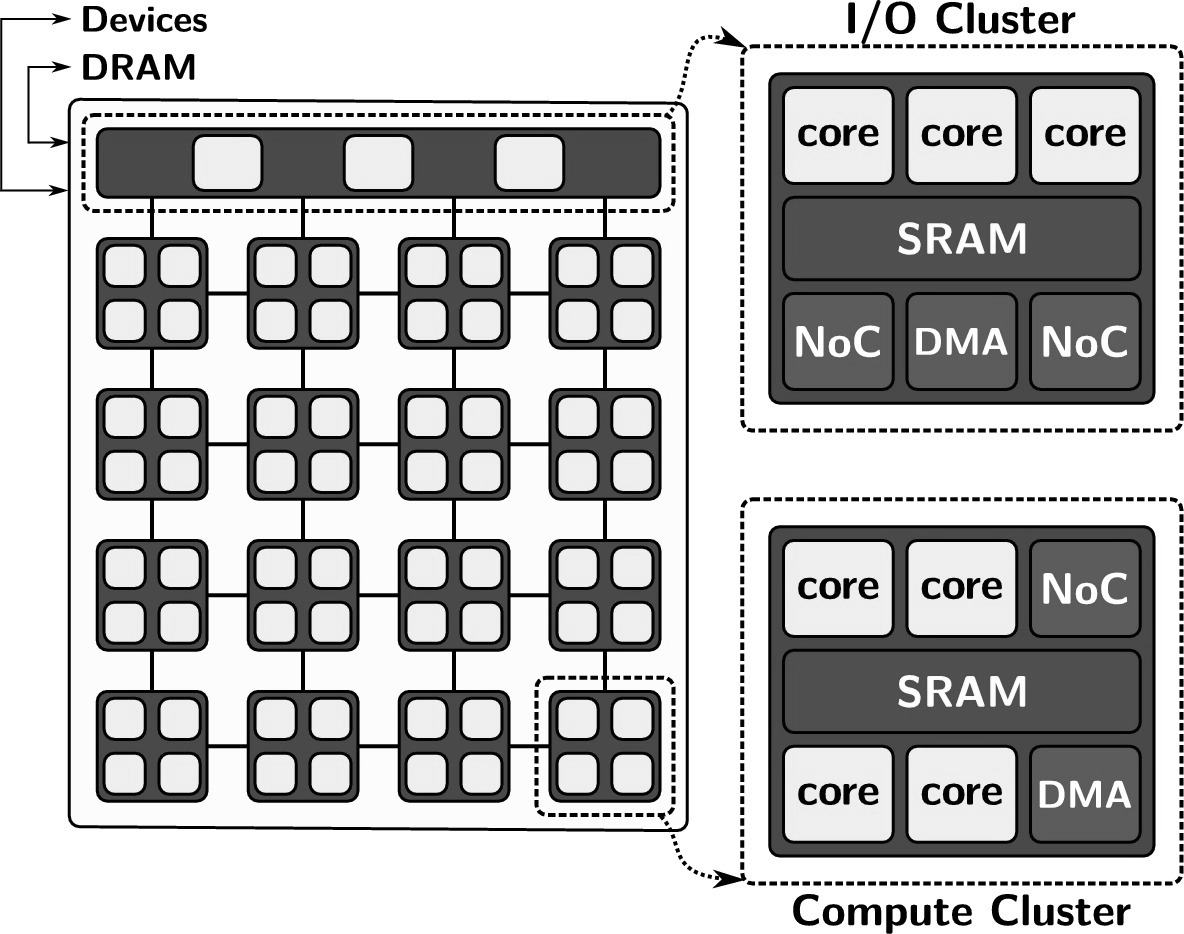
\includegraphics[width=0.5\linewidth]{content/images/lw-overview-gs.jpg}
	\caption{Visão conceitual de um processador \lw~\cite{penna2021inter}}
    \label{fig.lw-overview}
\end{figure}

Apesar dos processadores \lw serem uma alternativa às abordagens tradicionais no que se refere ao aumento de desempenho, as características arquiteturais introduzem severos problemas de programabilidade ao desenvolvimento de \software de aplicações paralelas~\cite{Castro-PARCO:2016}. Entre eles, podemos citar:

\begin{enumerate}[label= (\roman*)]
    \item Necessidade do uso de um modelo de programação híbrida que força troca de informação entre os \clusters exclusivamente por troca de mensagens via \noc enquanto a comunicação interna em um \cluster ocorre sobre memória compartilhada~\cite{kelly2013};
    \item Presença de um sistema de memória distribuída restritivo, formado por múltiplos espaços de endereçamento, exige o particionamento do conjunto de dados em blocos pequenos para manipulação nas pequenas memórias locais. A manipulação deve ocorrer um bloco de cada vez, necessitando a troca explicita de blocos com uma memória remota~\cite{Castro-PARCO:2016};
    \item Maiores latências e gargalos de comunicação através da \noc comparado com comunicação em memória compartilhada;
    \item Falta de suporte de coerência de cache em \hardware para economia de energia, exiging do programador a gerência da cache via \software; e
    \item Configuração heterogênea do \hardware, como \clusters destinados a funcionalidades específicas (computação útil e I/O), dificulta o desenvolvimento de aplicações.
\end{enumerate}

Atualmente, estudos exploram soluções para amenizar o impacto das arquiteturais sobre o desenvolvimento de \software. \oss distribuídos sobresaem-se por proverem um ambiente de programação mais robusto e rico~\cite{asmussen_m3:_2016, kluge_operating_2014, penna:sbesc19}. Dentre essas soluções, o modelo de um \os distribuído baseado em uma abordagem \multikernel descata-se por aderir a natureza distribuída e restritiva dos \lws~\cite{penna2017-1,penna2017-2,penna2019}.

Nesse cenário, a virtualização dos recursos do processador é importante para o suporte a multi-aplicação e melhor uso do \hardware disponível~\cite{vanz2022virtualizaccao}. Contudo, as características arquiteturais dos \lws, especialmente relacionadas à memória, inviabilizam um suporte complexo para virtualização. Por exemplo, máquinas virtuais utilizadas em ambientes \cloud possuem à disposição centenas de GBs de memória para isolar duplicatas inteiras do \os com a ajuda de virtualização a nível de instrução~\cite{sharma2016containers}. Nos \lws, as pequenas memórias locais e a simplificação do \hardware para reduzir o consumo energético restringem os tipos de virtualização suportados.

Neste contexto, este trabalho explora um modelo mais leve de virtualização para \lws baseado no conceito de contêineres. Contêineres são executados pelo \os como aplicações virtuais e não incluem um \os convidado, resultando em um menor impacto no sistema de memória e requisitando menor complexidade do \hardware~\cite{thalheim2018cntr, sharma2016containers}.

\section{Objetivos}
\label{sec.goals}

Com base nas motivações citadas previamente, os objetivos deste trabalho serão especificados nas próximas seções.

\subsection{Objetivo Principal}
\label{sec.goals.primary}

O objetivo principal deste trabalho é virtualizar os recursos internos de um \cluster de um \lw. Ao desvincular os recursos locais utilizados por um processo dentro do \nanvix, um \os para \lws, nós conseguiremos prover maior controle e mobilidade de processos no processador.

\subsection{Objetivos Específicos}
\label{sec.goals.secondary}

\begin{enumerate}[label= (\roman*)]
    \item Propor um modelo de virtualização adaptado às necessidades e restrições dos \lws;
    \item Implementar o modelo proposto no \nanvix, um \so distribuído para \lws;
    \item Analisar a corretude da solução através do desenvolvimento de \benchmarks que avaliem a migração de processos;
    \item Analisar o impacto do modelo de virtualização nos diversos níveis de abstração do \nanvix.
\end{enumerate}

\section{Organização do Trabalho}
\label{sec.organization}

Os próximos capítulos do trabalho estão organizadas da seguinte maneira. O \autoref{chap.background} apresenta conceitos fundameitais para o entendimento do trabalho, tais como um detalhamento da arquitetura dos \lws e do \nanvix. O \autoref{chap.related-work} discute os trabalhos relacionados. O \autoref{chap.dev.virtualizacao} expõe a proposta deste trabalho de conclusão e os detalhes de desenvolvimento da solução a ser implementada. O \autoref{chap.results} exibe e discute alguns resultados preliminares já obtidos. Por fim, o \autoref{chap.conclusions} apresenta as conclusões deste trabalho e pontua os próximos passos da pesquisa.

\chapter{Referencial Teórico}
\label{chap.background}

\section{Multiprocessadores}
\label{sec.multiprocessadores}

\section{Multicomputadores}
\label{sec.multicomputadores}

\todo{incluir base multiprocessadores/multicomputadores nesta seção}
\section{\Lws}
\label{sec.lw}

\section{\nanvix}
\todo{overview/threads/comunicação}
O \nanvix\footnote{Disponível em https://github.com/nanvix} é um \os distribuído e de propósito geral que busca equilibrar desempenho, portabilidade e programabilidade para \lws  \cite{penna:sbesc19}. \nanvix é estruturado em 3 camadas de \kernel. São elas:
\begin{enumerate}[label=(\roman*)]
    \item \nanvix \hal: é a camada mais baixa que abstrai os recursos de \hardware sobre uma visão comum;
    
    \item \nanvix \microkernel: é a camada intermediária que provê gerenciamento de recursos e os serviços mínimos de um \os em um \cluster;
    
    \item \nanvix \multikernel: é a camada superior que provê os serviços de um \os. Os serviços atendem as requisições vindas dos processos de usuário através de um modelo cliente-servidor;
\end{enumerate}
    
Em sua abordagem original, os processos no \nanvix são estáticos, \ie cada \cluster possui apenas um processo. Desse modo, uma vez que o processo inicia sua execução em um \cluster, este finalizará a execução no mesmo \cluster. 
Isso torna o processo dependente do \cluster que o executa \eg a comunicação entre processos está atrelada aos \clusters nos quais os processos são executados e não aos processos em si. A falta de mobilidade dos processos nesse modelo pode trazer sobrecargas ao processador e afeta o suporte a multi-aplicação. Por exemplo, a comunicação entre \clusters próximos é mais rápida e resulta em menor consumo energético do processador. Sendo assim, melhorar a mobilidade e a disposição dos processos no processador \ie viabilizar a migração de processos entre \clusters, possibilitaria melhorar o gerenciamento dos recursos do mesmo.

\todo{trocar por entrada no glossário}
\section{\nanvix \textit{Hardware Abstraction Layer} (HAL)}
\label{sec.nanvixhal}

\subsection{\nanvix \microkernel}
\label{sec.nanvixmicrokernel}

\subsection{\nanvix \multikernel}
\label{sec.nanvixmultikernel}

\section{Virtualização e Conteinerização}
\label{sec.virtualização}

\glsresetall
\chapter{Trabalhos Relacionados}
\label{chap.related-work}

Neste capítulo, serão mostradas técnicas e pesquisas que estão sendo desenvolvidas no que diz respeito à virtualização e migração. Serão apresentados trabalhos relacionados, bem como serão evidenciadas as semelhanças e diferenças com o presente trabalho.

Grande parte das pesquisas relacionadas à migração estão inseridas em ambientes \cloud. Nesses casos, os esforços estão voltados para redução do tempo total de migração, diminuição do \downtime~\cite{migration-linux-conteiners,clark2005live} e exploração/otimização das vantagens que a migração de processos oferece nesses ambientes computacionais. Entre essas vantagens podem-se citar:
\begin{enumerate}[label=(\roman*)]
    \item Balanceamento de carga~\cite{live-vm-migration-techniques,ada-things};
    \item Tolerância a falhas~\cite{fernando2019live};
    \item Gerenciamento do consumo de energia~\cite{aldossary2018performance};
    \item Compartilhamento de recursos; e
    \item Manutenção de sistemas sem interrupções~\cite{live-vm-migration-techniques,ada-things}.
\end{enumerate}

Apesar da maioria das pesquisas estarem voltadas à exploração desses benefícios e diminuição do tempo de migração e \downtime em ambientes \cloud, há alguns autores preocupados com o desenvolvimento de soluções envolvendo virtualização e migração em ambientes de recursos restritos. Dessa forma, como a temática de limitação de recursos, especialmente de memória, é muito presente neste trabalho, serão abordados nos próximos parágrafos algumas pesquisas desses autores \ie pesquisas voltadas à busca pelo uso da virtualização/migração de forma mais leve e cujo impacto no \hardware seja reduzido, se adaptando a esses sistemas de recursos limitados.

\section{\textit{''Virtualization on TrustZone-enabled Microcontrollers? Voilà!''}}

O artigo \textit{''Virtualization on TrustZone-enabled Microcontrollers? Voilà!''}~\cite{pinto2019virtualization} adressa a possiblidade de implementação da virtualização em microcontroladores que utilizam \trustzone. \trustzone é uma tecnologia de \hardware voltada à segurança, em que a execução de um sistema pode ser dividida entre normal e segura. Os autores afirmam que essa tecnologia pode ser explorada além das suas propriedades de segurança. Isso porque o \trustzone também provê certo nível de isolamento dos recursos, o que o torna viável de ser usado para virtualização, afinal o isolamento cria um ambiente seguro e propício para a execução simultânea e isolada de múltiplas \vms.

O artigo expõe a dificuldade de se implementar a virtualização em \mcus devido aos seus recursos limitados. Nesses ambientes, não é possível a utilização de \hypervisors tradicionais, haja vista a baixa complexidade de \hardware das \mcus. Sendo assim, para atender a necessidade de baixo impacto nos recursos dos \mcus, os autores propõem uma solução que usa um \hypervisor mais leve para gerenciar as \vms nesses ambientes utilizando a tecnologia \trustzone para garantir o isolamento das \vms.

Os testes foram feitos num microcontrolador \textit{Cortex-M4}. Conforme descrito pelos autores, a solução, de fato, garante o suporte à execução múltipla de \vms em microcontroladores.

\section{\textit{''Checkpointing and migration of IoT edge functions''}}


O artigo \textit{''Checkpointing and migration of IoT edge functions''}~\cite{karhula2019checkpointing} propõe um artifício envolvendo migração de contêiners entre dispositivos \iot de borda como solução para a diminuição do uso de recursos em dispositivos \iot.

Os autores evidenciam que os aparelhos \iot são usados na computação de borda para provomover o que chamamos de \faas, que é um tipo de serviço oferecido por diversas plataformas, como a \textit{Amazon AWS Lambda} e \textit{Google Cloud Functions}. O problema é que esses dispositivos possuem recursos limitados, restringindo-se à execução de poucos contêineres simultaneamente. Além disso, as abordagens tradicionais de \faas sugerem a execução ininterrupta dos contêineres que são iniciados. Isso torna a computação de borda ineficiente, pois esse esquema pode sobrecarregar rapidamente os dispositivos \iot, haja vista a memória limitada desses. A situação se agrava ainda mais quando consideramos funções de longa duração bloqueantes (muito comuns em sistemas de autenticação) \eg funções que esperam alguma requisição, resposta ou qualquer tipo de sinal de outro sistema, seja ele um outro dispositivo \iot ou uma ação humana.

Dessa forma, os autores propõe um esquema de \checkpointing utilizando \docker e \criu. Através dessas tecnologias, os contêineres que não estão executando computação útil são interrompidos e salvos em disco, liberando espaço da memória para a execução de outro contêiner. Isso se torna extremamente útil quando consideramos funções de longa duração bloqueantes, já que durante o tempo de espera pelo sinal, a aplicação pode ser interrompida. Além disso, com o estado salvo em disco, a migração de contêineres entre dispositivos \iot de borda se torna possível. Dessa forma, além de reduzir o uso de recursos nos dispositivos de computação em borda, através da migração dos contêineres, outros benefícios surgem, como o balanceamento de carga e tolerância a falhas entre aparelhos \iot de borda.

Os testes foram feitos em uma \textit{Raspberry Pi 2 Model B}, a qual rodava diversos contêineres com aplicações em \textit{Node JS} de longa duração e que simulavam o comportamento bloqueante. Os resultados apontam que houve economia no uso de recursos, em especial da memória e que a migração de contêineres entre dispositivos \iot de borda é possível.

\section{ \textit{''Lightweight virtualization as enabling technology for future smart cars''}}

O artigo \textit{''Lightweight virtualization as enabling technology for future smart cars''}~\cite{smartcarslwvirtualization} discorre sobre a possibilidade de usar a virtualização no desenvolvimento de apĺicações para carros inteligentes. Os sistemas presentes nos carros inteligentes também tem certa limitação de recursos que dificultam a aplicação direta de \hypervisors tradicionais, muito comuns em ambientes \cloud.

Sendo assim, os autores propõem um sistema que utiliza contêineres \docker para criar uma camada de abstração a nível de processo. Dessa forma, cada aplicação é executada em um contêiner distinto. Esse sistema tem impacto menor nos recursos de \hardware e é suficiente para garantir a execução isolada das aplicações virtuais (contêineres).

Além disso, o sistema engloba um escalonador de contêineres, que é responsável por gerenciar os contêineres e o \hardware alocado para cada um. Além disso, tem finalidade de sinalizar a instanciação e destuição dos contêineres conforme a necessidade. Esse escalonador é capaz de gerenciar os recursos de \hardware de forma a garantir que os contêineres sejam executados de maneira eficiente, sem que haja desperdício de recursos. No modelo proposto pelos autores, há 4 tipos de tarefas: \critical, \high, \moderate e \low. Cada um desses tipos possui um nível de prioridade, sendo que a \critical é o mais prioritário e o \low é o menos prioritário. O escalonador é responsável por garantir que as tarefas de maior prioridade sejam executadas primeiro. Tarefas relacionadas à segurança dos passageiros \eg sistemas de alerta ou câmera são consideradas mais prioritárias que tarefas relacionadas à sistemas de entretenimento \eg sistemas de áudio ou vídeo.

A proposta foi testada em uma \textit{Raspberry Pi 3} e os resultados foram considerados positivos. Os contêineres garantiram a execução do sistema de maneira a considerar a limitação de \hardware e suportaram a execução paralela de múltiplas aplicações. O escalonador de contêineres foi capaz de gerenciar os recursos de maneira eficiente, priorizando as tarefas de maior prioridade.

\section{Comparação do Presente Trabalho com os Trabalhos Relacionados}

O presente trabalho se asemelha com os trabalhos relacionados apresentados no sentido de aplicar a virtualização e migração em um sistema com recursos restritos. Contudo, em contraste com os trabalhos apresentados, a principal vantagem explorada com a virtualização é o aumento da mobilidade dos processos, possibilitando a migração de processos. A utilização eficiente dos recursos promovida pela virtualização, mesmo que necessária nos \lws pela limitação de recursos computacionais (em especial a memória) se torna uma vantagem indireta da virtualização. Isso porque o uso eficiente de \hardware é provido mais pela migração (através da melhor disposição dos processos entre os \clusters) do que pela virtualização em si.

Além disso, o presente trabalho explora a virtualização e migração usando contêineres, tal qual o segundo e terceiro trabalho, porém em um ambiente diferente e com outra abordagem. Neste trabalho, o foco é o desenvolvimento de um sistema de virtualização baseado em contêineres adaptado ao \so e sem o uso de ferramentas externas, como o \docker. Além disso, a migração das aplicações são entre \clusters de um mesmo processador, e não entre nós de computação de borda ou servidores \cloud.



% Os autores costumam aliar uma ou mais das características citadas acima para desenvolverem suas pesquisas. Por exemplo:

%     Para evitar que muitos usuários tenham que fazer requisições à aplicações hospedadas em servidores distantes ou com muito tráfego, pode-se utilizar a transparência de localidade de execução de aplicações com a manutenção destas sem sua suspenção. Assim, é possível explorar algorítmos ou modelos para melhor posicionar as aplicações na rede com o objetivo de atender a maior quantidade de usuários, de maneira mais eficiente e sem que o sistema precise ser desligado~\cite{live-migration-sdn}. Ademais, esses modelos podem ser especializados para tipos específicos de aplicações, como \iot~\cite{ada-things}.

%     Além disso, pesquisas são feitas com o intuito de tornar a migração de \vms entre servidores tolerante a falhas~\cite{fernando2019live}. A migração de \vms por algum motivo pode falhar (devido a problemas de rede, por exemplo). Nesse contexto, alguns autores sugerem o uso de \checkpoints, os quais são estados consistentes da \vm em dado momento. Se a migração falhar, a \vm pode ser restaurada para um \checkpoint. Isso evita que a \vm seja perdida.

% Em contraste com os trabalhos apresentados, nossa proposta não está inserida em ambientes \cloud. Seu foco está na migração de processos entre \clusters em um mesmo \chip, em um sistema computacional restritivo que restringe as técnicas possíveis a serem utilizadas. Além disso, nosso trabalho se difere dos demais trabalhos por explorar a virtualização e migração de processos inserida no contexto dos \lws e não apenas buscando otimizar algoritmos específicos, \eg \livemigration.
\glsresetall
\chapter{Proposta de Virtualização e Migração de Processos para \textit{Lightweight Manycores}}
\label{chap.dev.virtualizacao}

Este trabalho de conclusão propõe-se a aumentar a independência dos processos no processador através do projeto e desenvolvimento do suporte à virtualização e migração de processos em \lws. Ambientes \cloud, nos quais o sistema de memória é de alta capacidade, usufruem da utilização de \vms para isolar duplicatas inteiras de \oss com o auxílio da virtualização a nível de instrução~\cite{sharma2016containers}. Em oposição, \lws não dispõem de centenas de GBs de memória, mas sim pequenas memórias locais. Isso associado a outras simplificações de \hardware faz com que algumas técnicas de virtualização sejam impraticáveis nesses ambientes computacionais.


Nesse contexto, visando atenuar o impacto da virtualização no sistema de memória, o presente trabalho explora um modelo de virtualização mais leve, baseado em contêineres adaptado para \lws. O \so executa os contêineres como aplicações virtuais. Sendo assim, não há a necessidade de um \os convidado, resultando em um menor impacto no sistema de memória e requisitando menor complexidade do \hardware~\cite{thalheim2018cntr, sharma2016containers}.


\section{contexto de um processo}
\mytodo{threads, memoria, syscall, comunicação, estruturas de sincronização}
\mytodo{conteinerização no nanvix}



\begin{figure}[t]
	\centering
	
	\subcaptionminipage[fig.nanvix.without-uarea]%
                   {.4\textwidth}
                   {\os sem isolamento.}
                   {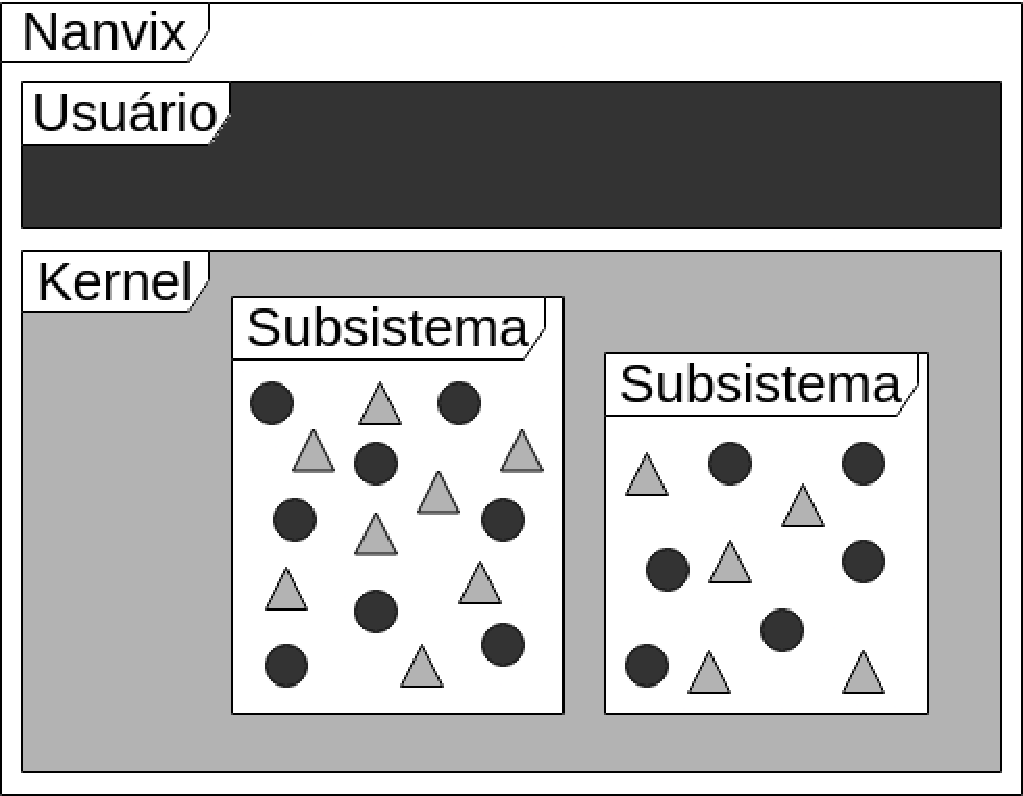
\includegraphics[width=\textwidth]{content/images/nanvix-without-uarea-uk.pdf}}
	\qquad
	\subcaptionminipage[fig.nanvix.with-uarea]
                   {.4\textwidth}
                   {\os com isolamento.}
                   {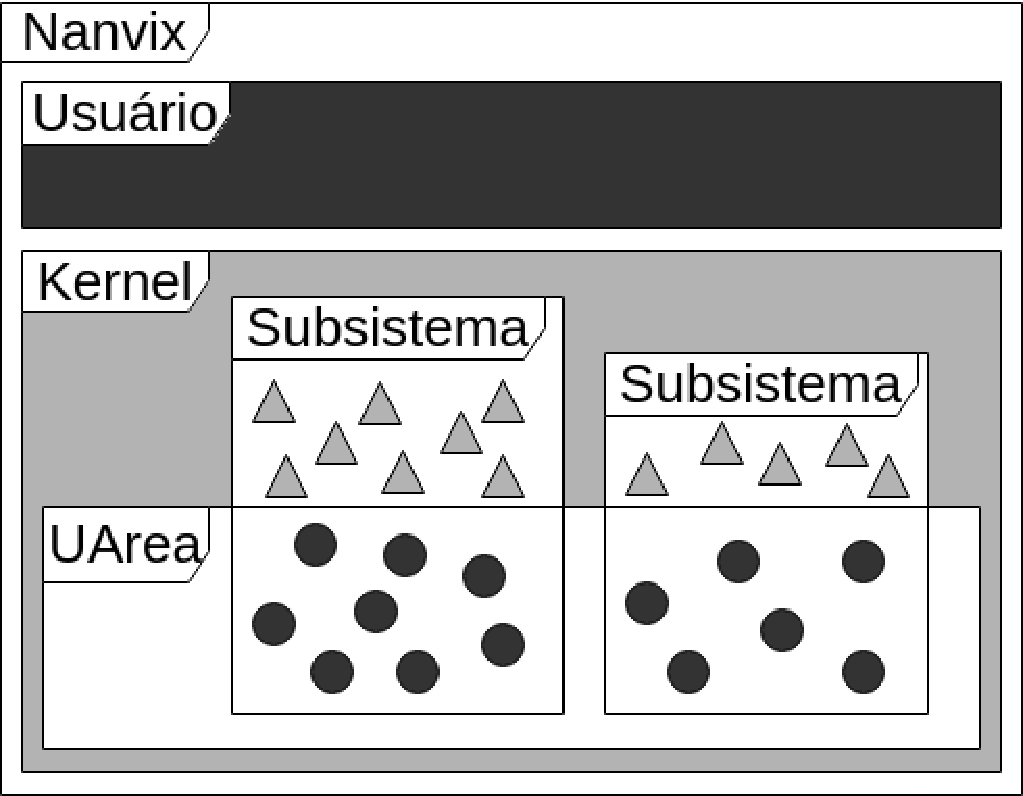
\includegraphics[width=\textwidth]{content/images/nanvix-with-uarea-uk.pdf}}

	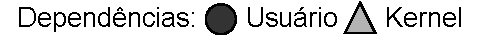
\includegraphics[width=.33\linewidth]{content/images/legenda.pdf}
	
	\caption{Diferença da estrutura do \nanvix com e sem a \textit{User Area}.}%
\end{figure}

\subsection{Isolamento do contexto de um processo de usuário}
\label{sec.dev.kernel-usuario}

\subsubsection{Divisão de Dados e Instruções}
\label{sec.divisao-dados-instrucao}

    Para a virtualização de processos através da conteinerização, é recomendável que as informações relevantes para a manipulação dos processos em execução estejam isoladas das informações internas do próprio \os para que os recursos de \hardware sejam utilizados de maneira eficiente~\cite{live-vm-migration-techniques}.
    A \autoref{fig.nanvix.without-uarea} ilustra como os subsistemas do \nanvix são originalmente estruturados. Não há uma divisão explícita do que são dados para funcionamento interno do \os ou dependências locais do processo.
    Esta abordagem torna algumas das funcionalidades do \os onerosas porque ela dificulta o acesso às informações do processo e impacta partes independentes do sistema, \eg migração e segurança dos processos.

    Além disso, a geração original de um executável do \nanvix compila todos os níveis em bibliotecas estáticas (\hal, \microkernel, \libnanvix, \ulibc e \multikernel) e as junta com a aplicação do usuário de forma a misturar o que é \kernel do que é usuário.
    %
    Visando a separação das informações entre usuário e \kernel, nós adaptamos o \script de ligação original do \nanvix. Na nova versão, as seções .text, .data, .bss e .rodata dos arquivos binários compilados são renomeados, especificando qual camada de abstração tal arquivo pertence. Desta forma, é possível identificar dados e instruções de cada camada do \nanvix, assim como as informações do usuário. Sendo assim, são geradas seções .text, .data, .rodata e .bss específicas para o \kernel e usuário. Portanto, todas as informações de \kernel, alocadas nos endereços mais baixos da memória, são isoladas das informações de aplicação, alocadas nos endereços mais altos da memória. Neste processo, são exportadas algumas constantes que apontam onde começam e terminam as partes do binário que são relacionadas ao \kernel e à aplicação. Essas constantes permitem a manipulação e gerenciamento mais precisos dos segmentos de memória do \kernel e da aplicação.
    
    Através dessa estratégia, todos os \clusters passam a ter a mesma organização interna de \kernel, facilitando a migração. Ou seja, a migração pode ser feita através do salvamento dos dados e instruções da aplicação de um \cluster e restauração destes nas respectivas posições em outro \cluster. Essas posições são identificadas pelas constantes exportadas no processo de compilação. Com isso, evita-se manipulações mais complexas do processo como a busca em várias regiões de memória para montar o estado interno do processo.

    % \mytodo{colocar alguma parte do linker?}
    % \mytodo{Souto: ngm vai entender o código do linker mas seria legal colocar e discutir melhor sobre as constantes.}
    
\subsubsection{\textit{User Area}}
\label{sec.uarea}

    Além da separação de dados e instruções entre \kernel e aplicação, é necessário a identificação e separação das estruturas internas do \so que são manipuladas pelo usuário e constituem o estado interno do processo. Nesse contexto, é introduzido o conceito de conteinerização para isolar as dependências que o usuário possui dentro do \cluster. Ou seja, nós isolamos os dados que são gerenciados pelo \kernel mas pertencem ao contexto do processo de usuário. Neste contexto, nós isolamos tais dados em uma região de memória bem definida, denominada de \uarea. 

    Detalhadamente, a \uarea mantém informações sobre:
    \begin{enumerate}[label=(\roman*)]
        \item \Threads ativas, incluindo identificadores e contextos;
        \item Ponteiros para suas pilhas de execução; 
        \item Variáveis de controle e filas de escalonamento;
        \item Estruturas de gerenciamento de chamadas de sistema; e
        \item Estruturas de gerenciamento de memória (\eg sistema de paginação).
    \end{enumerate}

    Essa estrutura genérica foi projetada para englobar as várias arquiteturas suportadas pelo \nanvix. Além disso, a estrutura permite a modificação e expansão, não se limitando ao estado atual do desenvolvimento do \nanvix, para atender os objetivos de outros projetos que usufruam do \nanvix.

\section{Migração de Processos}
\label{sec.migracao}

Como aplicação direta do isolamento do processo, a migração de processos torna-se viável. Especificamente, nós eliminamos a necessidade de descobrir quais são e onde estão as informações que compõem o estado de um processo dentro do \nanvix através da criação de uma instância isolada do espaço do usuário via conteinerização, facilitando a transferência de seu contexto. Isso só é possível porque os \clusters possuem uma estrutura de \kernel idêntica (devido às mudanças desenvolvidas no processo de compilação detalhados na \autoref{sec.divisao-dados-instrucao}). Por este motivo, eliminamos o envio de dados redundantes entre \clusters referentes à instância local do \os, atenuando o impacto da migração sobre a \noc.

\subsection{Rotina de migração}
\label{sec.rotina-migracao}

Para a migração de um processo entre \clusters foi desenvolvida uma rotina de migração. A funcionalidade é similar ao \criu, ferramenta utilizada por \softwares de gerenciamento de contêineres como o Docker. Porém, a migração é executada por intermédio de \daemons do \os. Neste do projeto, implementamos o algoritmo \hotmigration para migração de processos. A técnica de \hotmigration migra a aplicação durante sua execução, copiando as páginas de memória e o estado de execução da aplicação e restaurando a aplicação depois da transferência completa dos dados. A seguir é detalhado o fluxo de execução da migração:

\begin{description}
	\item[1. Congelamento da execução do processo em um estado consistente.] \hfill
	
	Antes do envio da aplicação a outro \cluster, é necessário que o processo esteja em um estado consistente e estático. Isso significa que durante o processo de migração é preciso que todas as operações dele sejam pausadas. Isso é feito objetivando evitar inconsistências que podem ser causadas por condições de corrida \eg impedir perda de instruções, retornos de chamadas de sistemas, sinais de sincronização, etc. Para atingir esse estado consistente, a chamada de sistema \freeze é invocada. Esta é uma chamada de sistema que é tratada apenas pelo \mcore. Especificamente, esta chamada ativa uma variável interna do \so que impede o escalonamento de \threads de aplicação (\threads que não executam no \mcore) e envia um sinal de reescalonamento para todos os \scores, para que as \threads de usuário saiam de execução o mais rápido possível. Isso garante uma pausa na aplicação sem que o \so seja impedido de executar, o que é imprescindível para a migração, já que as informações do processo precisam ser enviadas pelas interfaces \noc do \cluster remetente, o que exige que o \so atenda às requisições de envio de dados. Após o travamento no escalonamento de \threads de usuário, novas chamadas de sistema requisitadas pela aplicação não podem ocorrer. Sendo assim, após a migração, o \cluster destinatário atenderá às chamadas não atendidas e reconhecerá as atendidas, pois as estruturas de sincronização e variáveis de retorno são migradas também durante o processo. Após o congelamento do escalonamento e a retirada das \threads de usuário dos \scores, o processo é considerado consistente e seu contexto está apto para ser migrado.

	\item[2. Transferência do contexto do processo entre \clusters.] \hfill
	
	Com o processo em um estado consistente, uma \task de sistema, que é executada no \mcore, é criada para o envio dos dados ao \cluster destinatário. Através das abstrações de comunicação \mailbox e \portal, as seções de dados e instruções do processo são enviadas ao \cluster destinatário. Logo após, a \uarea é enviada. O envio de dados, instruções e \uarea garantem que o contexto inteiro do processo seja enviado, possibilitando a retomada da execução no \cluster destinatário.

	\item[3. Restauração da execução do processo no \cluster destino.] \hfill
	
	Com o contexto do processo já no \cluster destinatário, a execução é restaurada. Isso é feito pela chamada de sistema \unfreeze, que descongela o escalonamento de \threads de usuário. Assim, a execução do processo continua normalmente, agora em outro \cluster.
\end{description}

\mytodo{detalhar como funcionam as tasks e threads em cada cluster: remetente e destinatario}
\mytodo{como funciona a migração para um cluster com nenhum processo alocado}
\glsresetall
\chapter{Metodologia de Avaliação}
Neste capítulo, será apresentado como a solução foi avaliada. Particularmente, as perguntas que guiaram o desenvolvimento dos experimentos desenvolvidos para analisar a virtualização e a migração de processos no \nanvix foram:

\begin{enumerate}[label=(\roman*)]
    \item Qual o impacto do isolamento da \uarea e do código e dados de usuário sobre a execução do \nanvix?
    \item Qual a eficiência da migração de processos no \nanvix de acordo com a quantidade de estruturas manipuladas pela aplicação?
    \item Há sobrecarga no sistema de comunicação quando migramos apicações paralelamente?
\end{enumerate}

Para responder a primeira pergunta, foram desenvolvidos experimentos sobre a manipulação de \threads no \nanvix, que é o principal subsistema afetado pela \uarea. O experimento mensura os impactos na criação e junção de \threads através de diferentes perspectivas. Trata-se de um teste em que causamos um estresse no subsistema de \threads através da criação e junção do máximo de \threads que o sistema suporta. Especificamente, coletamos o tempo de execução, desvios e faltas ocorridas na \cache de dados e de instrução.

Para responder a segunda pergunta, foram desenvolvidos experimentos sobre a migração de processos no \nanvix. O experimento mensura o tempo de transferência de um processo entre \clusters de acordo com os recursos utilizados. Neste teste, variamos a quantidade de páginas de memória dinamicamente alocadas entre 0 e 32; e \threads usadas pela aplicação entre 1 e 17. Em resumo, neste experimento avaliamos como ocorre a progressão do tempo de transferência de um processo desde o mínimo de recursos utilizados (1 \thread e 0 páginas dinamicamente alocadas) até o máximo (17 \threads e 32 páginas dinamicamente alocadas).

Para responder a terceira pergunta, foi feito outro teste que mensura o \downtime da aplicação em diversos cenários. Neste teste, mensuramos o \downtime variando a quantidade de processos migrados paralelamente desde o mínimo (1 processo, envolvendo 2 \clusters) até o máximo (8 processos, envolvendo 16 \clusters).

Adicionalmente, um quarto teste foi feito com o objetivo de garantir a capacidade do \daemon suportar múltiplas migrações. Neste experimento, um processo é migrado de \cluster em \cluster até que percorra todos os \clusters do processador \ie o processo é migrado realizando um movimento circular, passando do \cluster 0 para o 1, do 1 para o 2, e assim sucessivamente até retornar ao \cluster 0.

Todos os testes foram realizados no processador \mppa. Realizamos múltiplas replicações para garantir maior confiança estatística (100 replicações para o primeiro experimento e 20 replicações para o segundo e terceiro experimento). Para a medição de tempo no segundo e terceiro experimento, utilizamos a abstração de comunicação \sync. Como as estruturas utilizadas por cada experimento variam, a quantidade de dados enviada também varia. Contudo, podemos generalizar a quantidade de \bytes enviada através da Equação \ref{eq.1}. Na Equação \ref{eq.1} o identificador \texttt{U} representa o tamanho do binário de usuário, \texttt{UA} o tamanho da \uarea, \texttt{SYSB} o tamanho da tabela de gerenciamento das chamadas de sistema, \texttt{PGDIR} o tamanho da tabela de diretórios de páginas, \texttt{PGTAB} o tamanho da tabela de página, \texttt{KSIDS} o tamanho da lista de gerenciamento de páginas de \kernel, \texttt{KSPHYS} a soma do tamanho das páginas de \kernel em uso, \texttt{FBMP} o tamanho do \bitmap de gerenciamento dos \frames e \texttt{FPHYS} a soma do tamanho dos \frames usados pela alocação dinâmica de páginas de memória.

\begin{equation}\label{eq.1}
    U + UA + SYSB + PGDIR + PGTAB + KSIDS + KSPHYS + FBMP + FPHYS
\end{equation}

Algumas dessas variáveis são constantes nos experimentos. Substituindo-as pelos seus respectivos valores em \bytes obtemos a Equação \ref{eq.2}.

\begin{gather}
    10608 + 2112 + 1920 + 4096 + 4096 + 160 + KSPHYS + 16 + FPHYS\\
    23008 + KSPHYS + FPHYS\label{eq.2}
\end{gather}

Sendo assim, percebemos que a quantidade de dados enviada varia em função da quantidade de páginas de \kernel em uso e da quantidade de páginas alocadas dinâmicamente. Tendo em vista que as variáveis do experimento são a quantidade de \threads e a quantidade de páginas alocadas dinamicamente, é importante entender como essas variáveis impactam em \texttt{KSPHYS} e \texttt{FPHYS}. Em mais detalhes, quando uma \thread é criada, duas páginas de \kernel são alocadas para esta nova \thread: uma para a pilha de execução em espaço de usuário; e outra para a pilha de execução em espaço de \kernel. Já quando uma página de usuário é dinamicamente criada, aumentamos o espaço do usuário em mais uma página \ie aumentamos o \texttt{FPHYS} em uma página (4096~B). Além disso, quando alocamos a primeira página de usuário, uma página de \kernel é utilizada como tabela de páginas para essa e as possíveis novas páginas a serem alocadas. Arranjando esses dados na Equação \ref{eq.2}, obtemos:

\[
\begin{cases}
    23008 + 4096(2*NTHREADS),& \text{se } NPAGES= 0\\
    23008 + 4096(2*NTHREADS + NPAGES + 1),& \text{se } NPAGES > 0
\end{cases}
\]
ou simplesmente:
\begin{equation}\label{eq.3}
    23008 + 4096(2*NTHREADS + NPAGES + min(P, 1))
\end{equation}

Onde \texttt{NTHREADS} é a quantidade de \threads criadas e \texttt{NPAGES} a quantidade de páginas criadas.


Quanto ao funcionamento dos experimentos, em resumo, no início do teste todos os \clusters sincronizavam entre si através do \sync. Neste momento, o \iocluster iniciava uma contagem de ciclos. Ao final do experimento, todos os \clusters envolvidos sincronizavam novamente. Neste momento, o \iocluster parava a contagem de ciclos e esse era o tempo que a migração demorou até seu término. Destaca-se que nos experimentos que precisavam de algum \setup inicial, o tempo de \setup não foi considerado. Por exemplo, no segundo experimento, o tempo para a criação de \threads, alocação e manipulação das páginas dinamicamente alocadas não é contabilizado no tempo final. O resultado, portanto, engloba apenas o \downtime da aplicação.



\chapter{Resultados Experimentais}
\label{chap.results}

% A solução foi avaliada em etapas anteriores ao desenvolvimento atual do trabalho e os resultados seguintes englobam apenas o susbsistema de \threads do \nanvix. 
% \todo{Seria bom colocar um capítulo de metodologia com perguntas que gostariamos de responder e detalhamento dos experimentos}
% %
% Para avaliar o impacto das mudanças feitas para a virtualização, foram desenvolvidos experimentos sobre a manipulação de \threads e suporte à migração de processos no \nanvix. Todos os experimentos foram executados no processador \mppa e os resultados mostrados são valores médios de 100 replicações de cada experimento para garantir 95\% de confiança estatística, resultando em um desvio padrão inferior a 1\%.
\begin{figure}[tb]
	\centering
	\subcaptionminipage[fig.fork-join]%
                   {.5\textwidth}
                   {Tempo de criação de \threads.}
                   {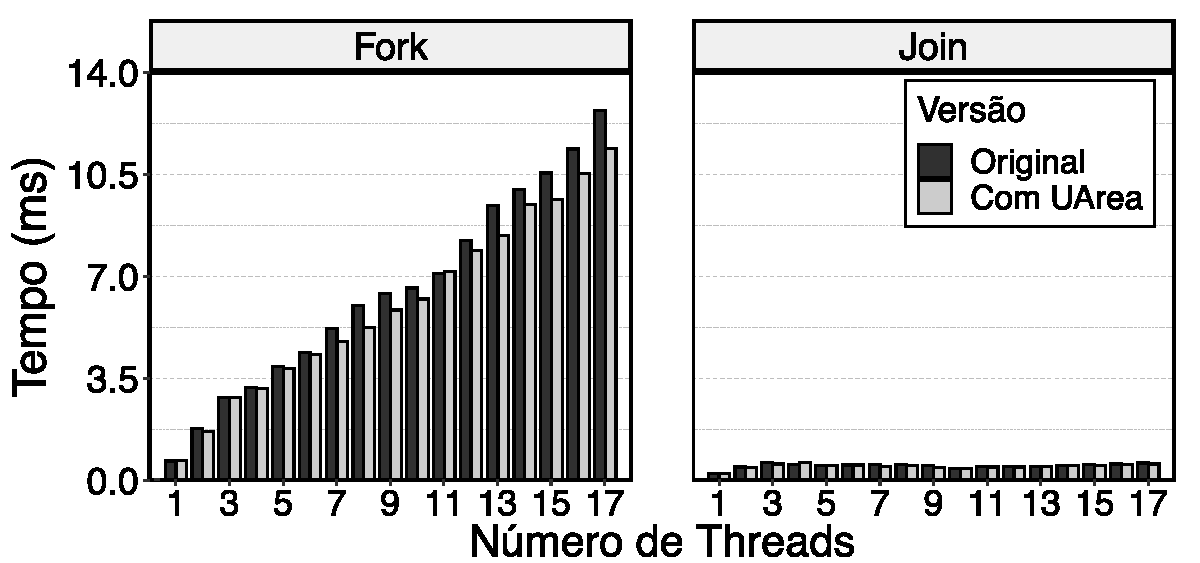
\includegraphics[width=\textwidth]{content/images/fork-join-kernel-time-bars.pdf}}
	\qquad
	\subcaptionminipage[fig.kernel-counters]
                   {.4\textwidth}
                   {Métricas do \kernel.}
                   {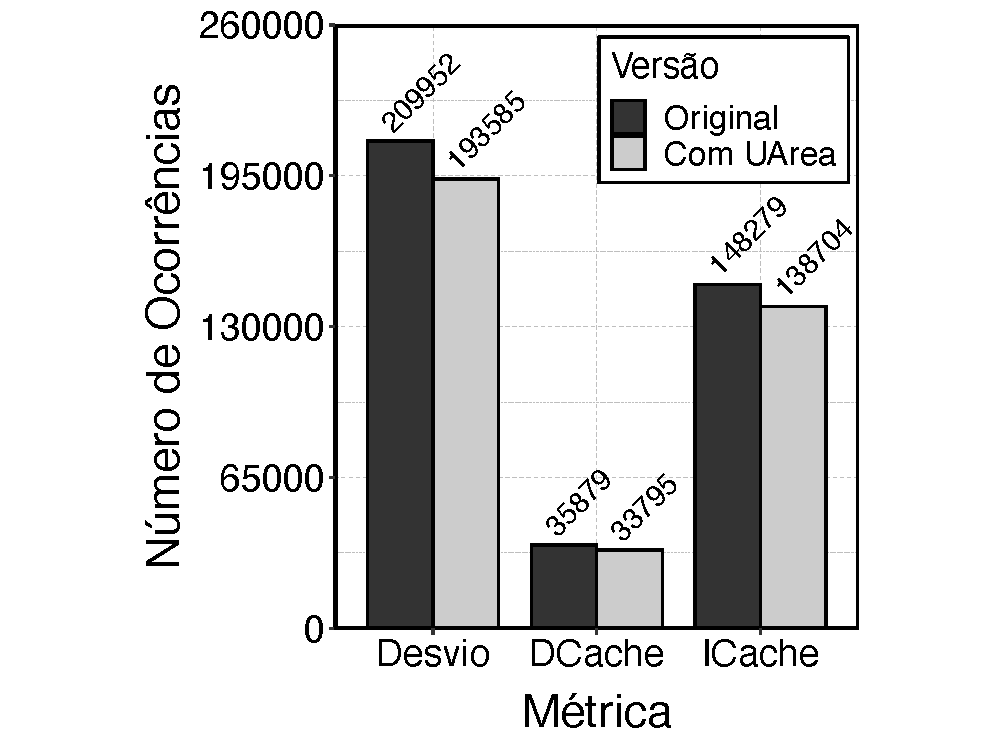
\includegraphics[width=\textwidth]{content/images/fork-join-kernel-counters.pdf}}
	\caption{Impactos da virtualização sobre a manipulação de \threads.\label{fig.threads}}%
\end{figure}

\begin{figure}[tb]
    \centering
    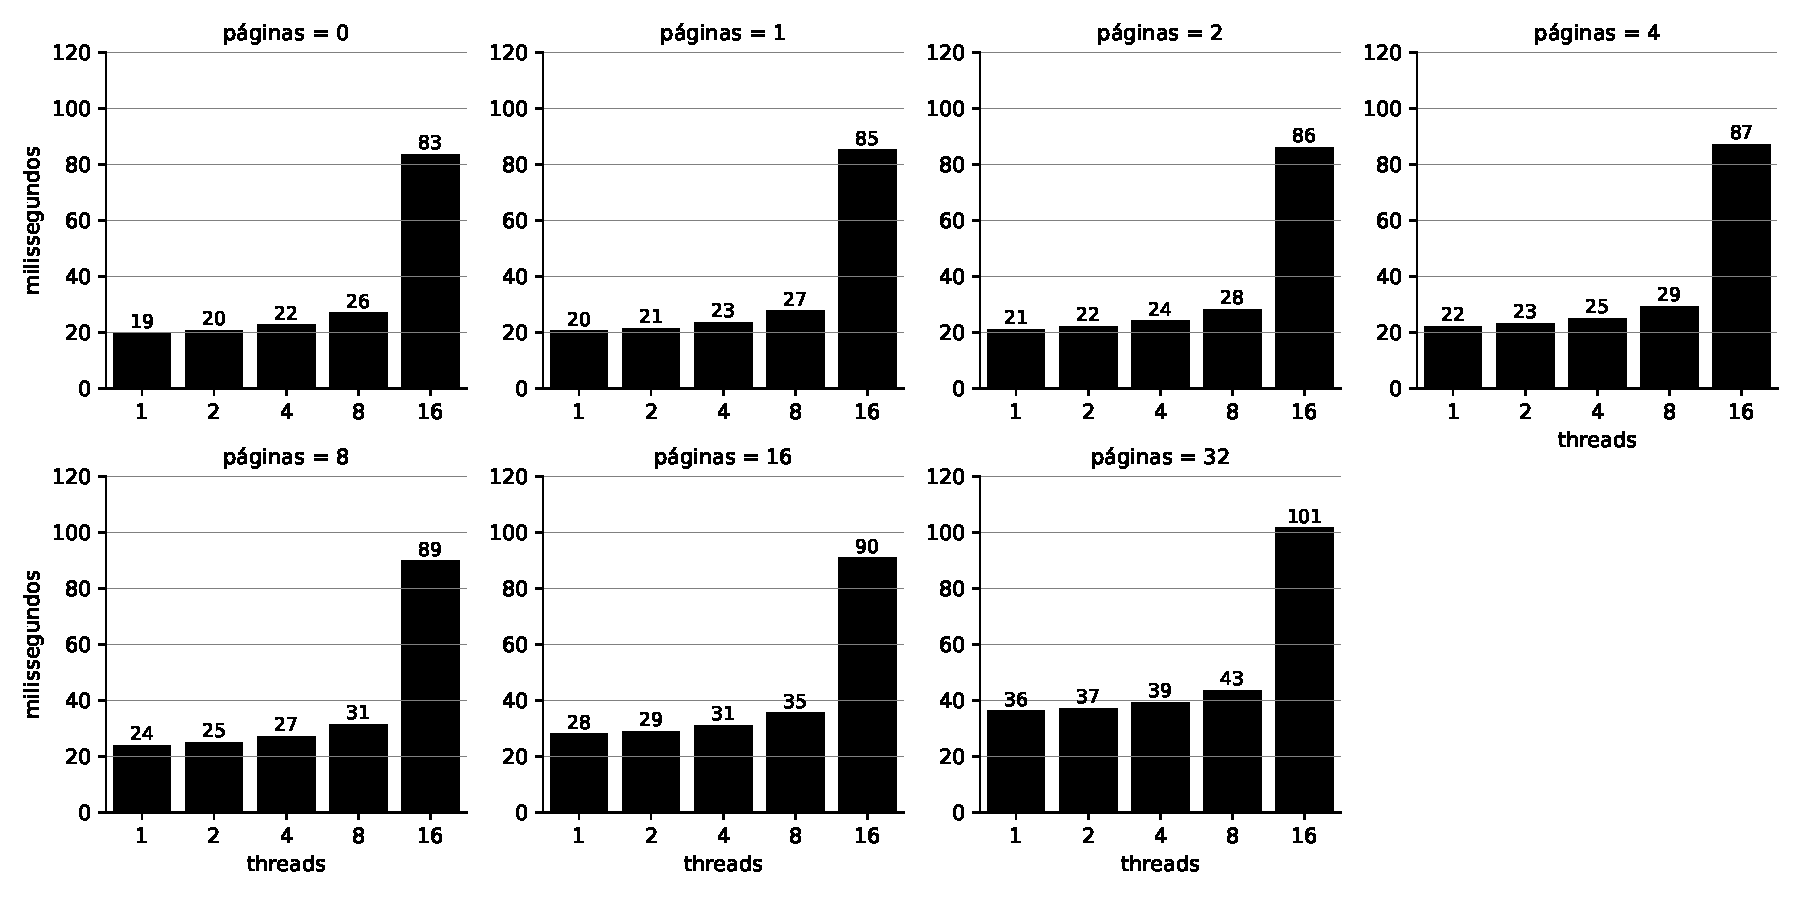
\includegraphics[width=\linewidth]{content/images/multiple_threads_pages.pdf}
    \caption{\Downtime da aplicação durante o experimento de migração fixando a quantidade de páginas alocadas dinamicamente}
    \label{fig.mtpages}
\end{figure}

\begin{figure}[tb]
    \centering
    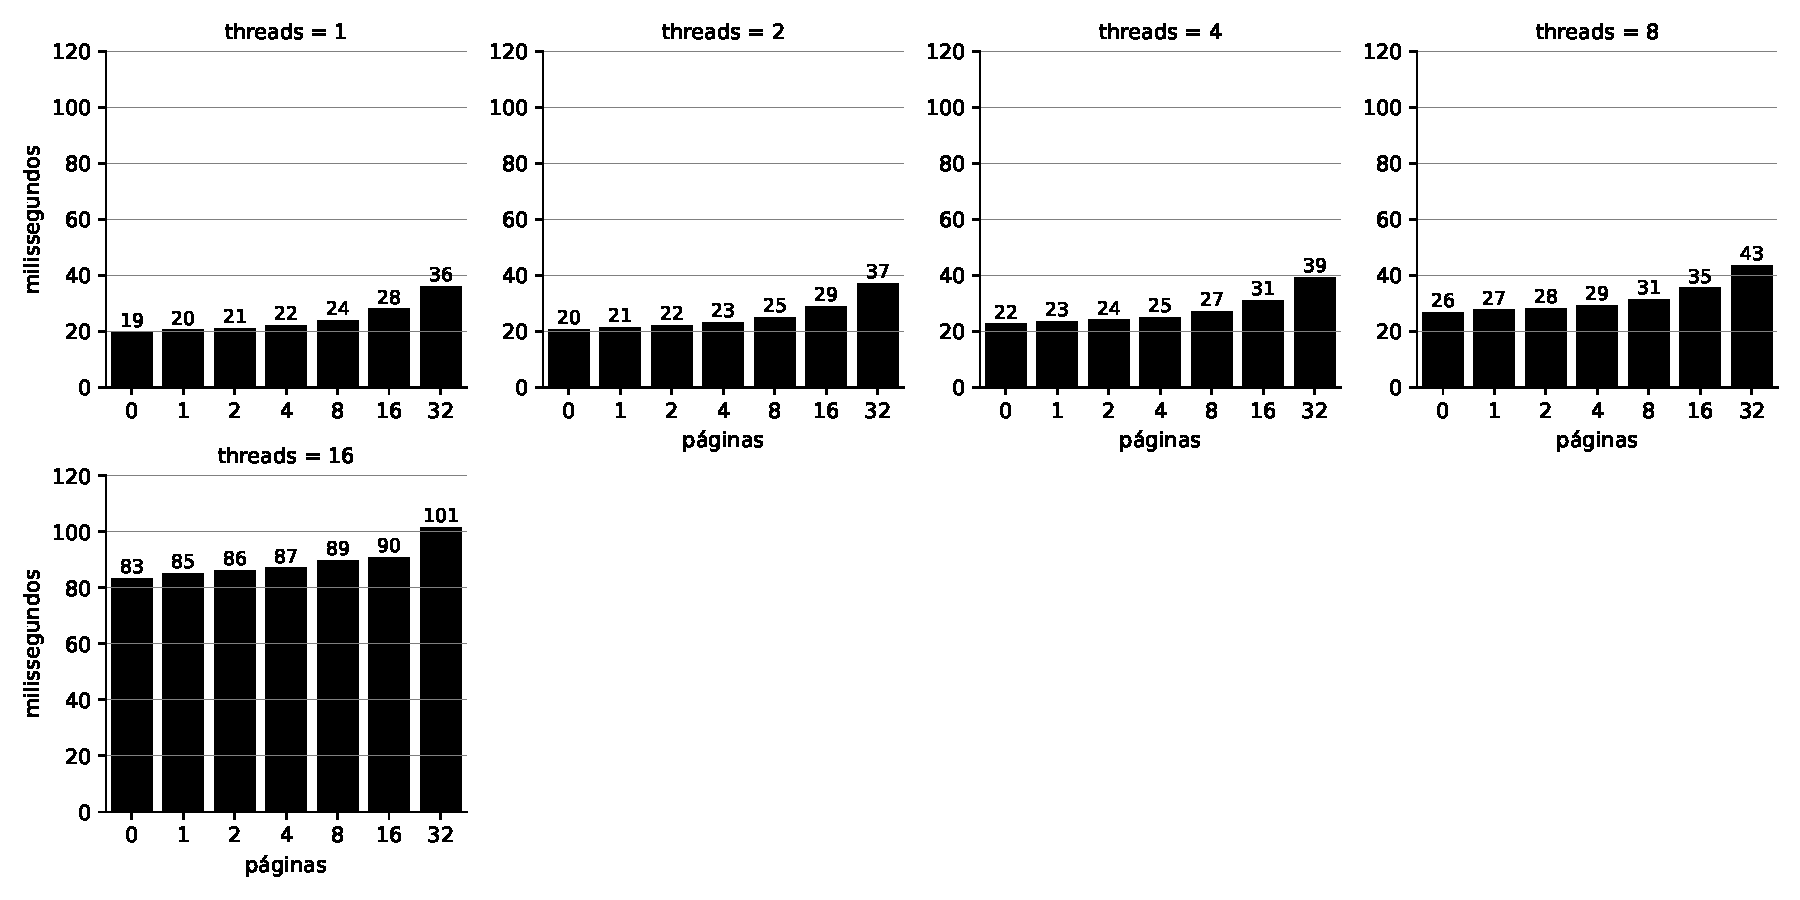
\includegraphics[width=\linewidth]{content/images/multiple_threads_threads.pdf}
    \caption{\Downtime da aplicação durante o experimento de migração fixando a quantidade de \threads}
    \label{fig.mtthreads}
\end{figure}

O primeiro experimento, o qual mensurava o impacto do isolamento da aplicação através da \uarea e separação do binário de usuário e \kernel, mostrou que o subsistema de \threads foi positivamente afetado. A \autoref{fig.fork-join} ilustra que o \nanvix obteve um leve ganho de desempenho nas operações de criação e junção de \threads. A \autoref{fig.kernel-counters} mostra a origem do aumento da performance. Percebemos que houve uma diminuição na quantidade de faltas em \cache (tanto de dados como de instruções) e a quantidade de desvios é menor na versão do \nanvix com a \uarea. Isso ocorre porque a \uarea explora melhor a localidade espacial dos dados, já que os dados estão aglomerados em um espaço menor da memória. Como consequência disso, o número de faltas na \cache e de desvios diminui, resultando em um aumento de desempenho.

O segundo experimento, que mensura o \downtime da aplicação em cenários variando a quantidade de recursos utilizados, mostrou os seguintes resultados. A \autoref{fig.mtpages} e a \autoref{fig.mtthreads} mostram a progressão de tempo sobre diferentes perspectivas (fixando-se as páginas e \threads, respectivamente). Como o esperado, o \downtime aumenta quanto maior for o número de páginas e \threads. Além disso, a quantidade de \threads se destaca por apresentar maior expressividade no tempo contabilizado em comparação com a quantidade de páginas. Isso acontece porque uma \thread acarreta em mais dados migrados do que uma página. De maneira geral, o \downtime é aproximadamente descrito pela função \ref{eq.downtime}:

\begin{equation}\label{eq.downtime}
    \begin{split}
        f(p, t) = \frac{17}{32}*p+t+18
    \end{split}
\end{equation}

Essa função descreve relativamente bem a progressão de tempo até 15 \threads. Como podemos observar nos gráficos, com 16 \threads há uma disparidade com a natureza aparentemente linear que a progressão de tempo aparenta ter. Isso acontece porque o \mppa possui 16 \cores por \cluster, o que significa que simultaneamente apenas 15 \threads de usuário podem executar, já que em um \core executam apenas \threads de sistema, que são responsáveis pelo tratamento de chamadas de sistema e execução das \tasks. Portanto, essa disparidade numérica que os gráficos apresentam são justificados pelo tempo extra que o teste ocupa com gerenciamento de \threads. Isso porque o teste finaliza com a junção de todas as \threads criadas no \cluster destinatário e tal processo exige tempo extra quando a quantidade de \threads é maior que 15, uma vez que algumas \threads precisariam esperar outras terminarem para poderem executar e, finalmente, finalizar sua execução.

O terceiro experimento, que mensurava o \downtime da aplicação quando múltiplas migrações aconteciam simultaneamente, mostrou que a quantidade de migrações paralelas não impacta significativamente o tempo. É importante destacar que nesse experimento foram migradas aplicações que usavam o máximo de recursos de sistema. Mesmo assim, a quantidade de dados não foi suficiente para impactar no \downtime.

Já o quarto experimento, o teste adicional que visava a comprovação da corretude do \daemon, mostrou que: o \daemon é capaz de ser reusado no mesmo \cluster diversas vezes independentemente do papel do \cluster na migração; e que é possível um processo ser migrado diversas vezes para diferentes \clusters, até em movimento circular envolvendo todos os \clusters, como no experimento.
\glsresetall
\chapter{Conclusões}
\label{chap.conclusions}

Neste trabalho, foi explorado um modelo de virtualização leve baseado em contêineres que considera as restrições arquiteturais dos \lws, adaptando-se as suas restrições, principalmente relacionadas à memória. A virtualização proposta visa melhorar a mobilidade e gerenciamento de processos para \lws no contexto de em um \os distribuído, o \nanvix.
%

Os resultados mostraram que a virtualização nesses ambientes é possível, bem como a migração de processos entre os \clusters do processador. A migração não afeta significativamente o sistema de comunicação, sendo possível realizar múltiplas migrações simultaneamente, e provocou um \downtime relativamente baixo, já que evitamos o envio de dados redundantes \eg relacionados ao \kernel. O isolamento das dependências de um processo aumentaram o desempenho de operações do \kernel na execução normal do \so, em especial no subsistema de \threads.

\section{Trabalhos Futuros}
Como trabalhos futuros, pretende-se:

\begin{enumerate}[label=(\roman*)]
    \item Ampliar a virtualização, englobando o subsistema de comunicação;
    \item Habilitar a execução simultânea de múltiplas aplicações no processador e sua proteção;
    \item Implementar um escalonador no \nanvix que considere a melhor distribuição de processos entre os \clusters;
    \item Implementar um sistema de \checkpointing que torne possível guardar estados de processos em disco;
\end{enumerate}


    
    %%%%%%%%%%%%%%%%%%%%%%%%%%%%%%%%%%%%%%%%%%%%%%%%%%%%%%%%%%%%%%%%%%%%
    %%% Elementos pós-textuais                                       %%%
    %%%%%%%%%%%%%%%%%%%%%%%%%%%%%%%%%%%%%%%%%%%%%%%%%%%%%%%%%%%%%%%%%%%%
    
    \postextual
    \bibliography{references}

%\apendices
%
%\chapter{Artigo Científico}
%\label{chap:apendice}
%
%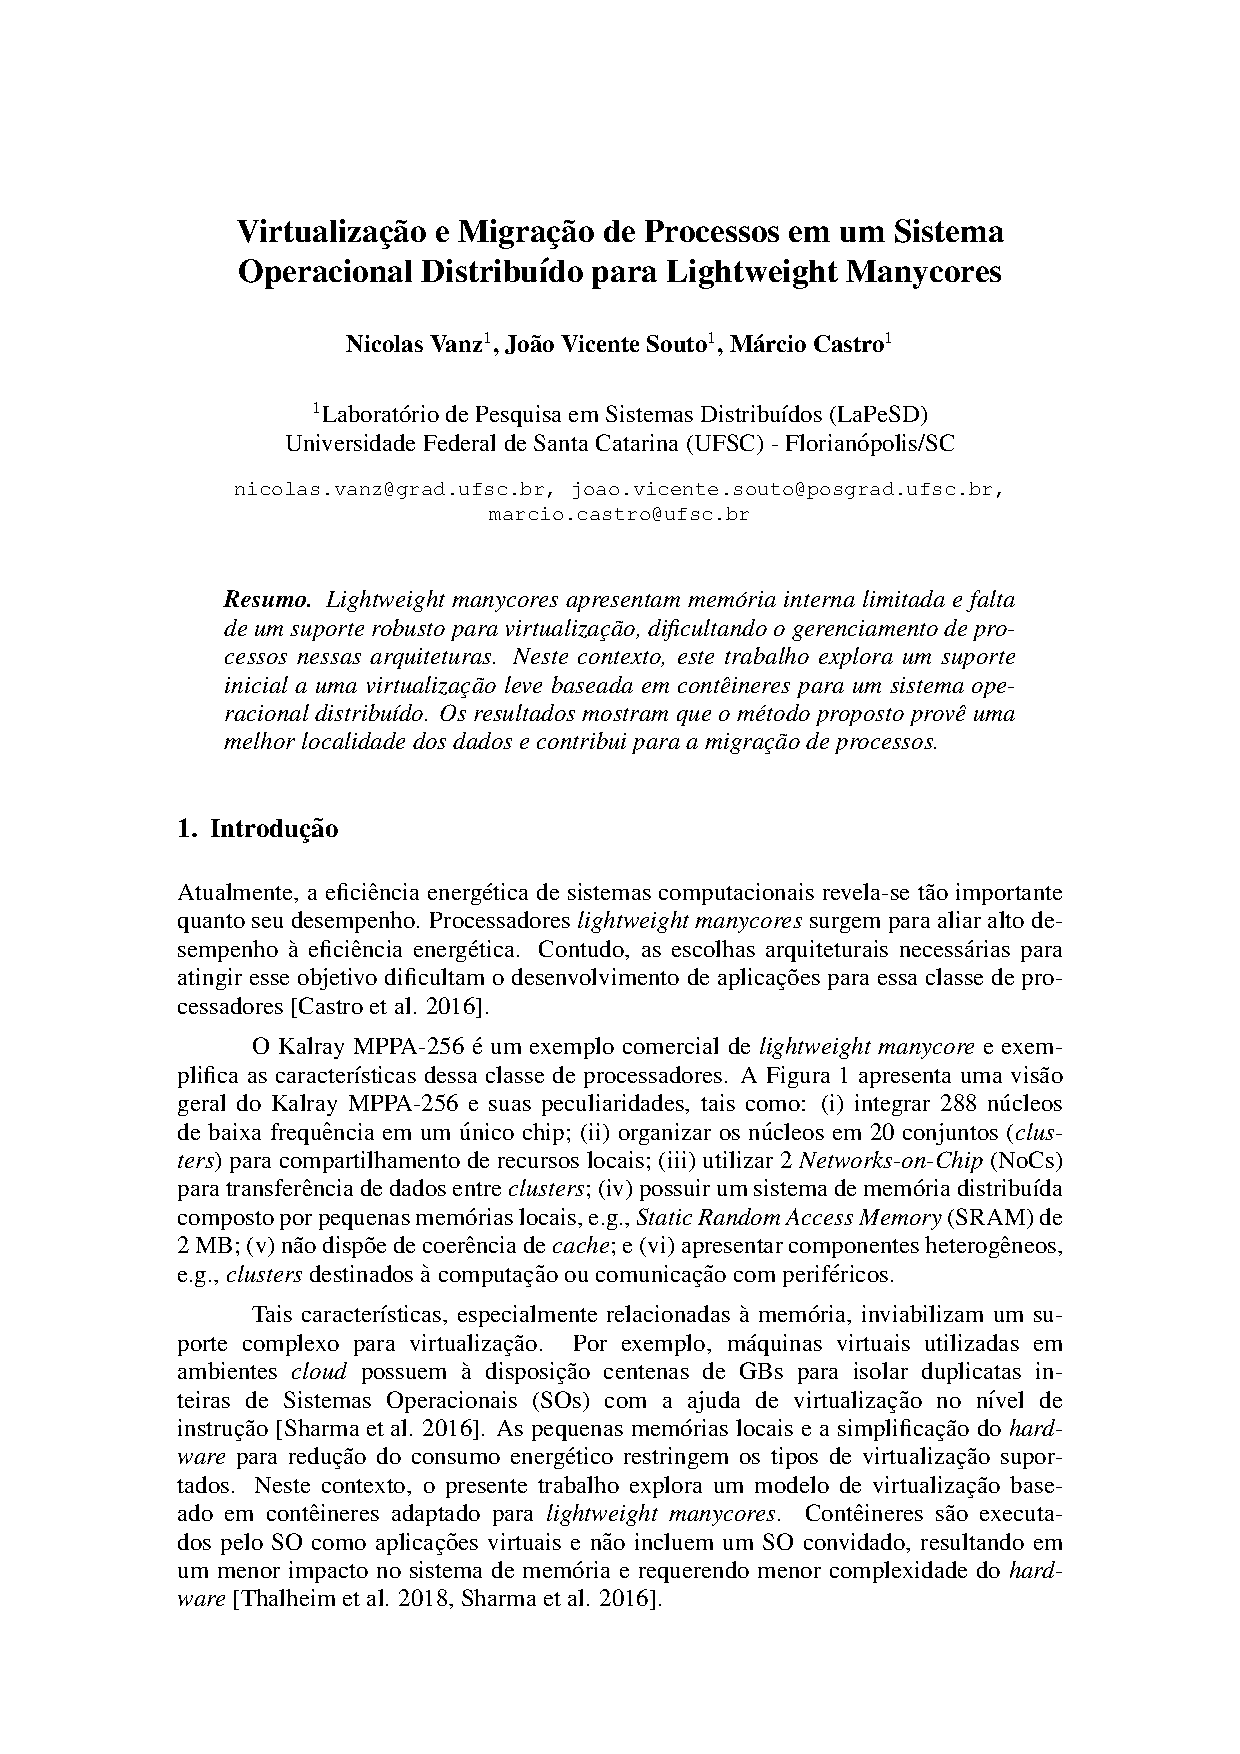
\includepdf[scale=1,pages=-,pagecommand={}]{content/apendices/erad.pdf}

% Uso de \cite em apêndice/anexo como se fossem antes do \bibliography{}.  NBR
% 14724 e NBR 6023, assim como os documentos da BU não especificam nada sobre
% citações dentro de apêndices/anexos. No entanto, em email trocado com a BU, a
% orientação foi de usar \cite{} normalmente e deixar que as referências sejam
% listadas na única bibliografia do documento, mesmo que esta esteja antes dos
% apêndices. A argumentação é que apêndices e anexos são numerados e fazem parte
% do documento, logo suas referências devem ser listadas como referências do
% documento. Além disso as normas não prevem segmentar as referências por
% capítulos.

    
\end{document}
